\documentclass[a4paper,parskip=half,DIV=14,BCOR=15mm]{scrreprt}
%\usepackage{showframe}

\usepackage[T1]{fontenc}
\usepackage{cmbright}
\usepackage[utf8]{inputenc}
\usepackage{hyperref}
\usepackage{graphicx}
\usepackage{microtype}
\usepackage{pgfgantt}
\usepackage{tabulary}
\usepackage[page]{appendix}
\usepackage{pdfpages}
\usepackage{multicol}
\interfootnotelinepenalty=10000

\usepackage{minted}
\renewcommand{\listingscaption}{\normalfont{}Listing}

\usepackage{booktabs}
\renewcommand{\arraystretch}{1.3}

% https://tex.stackexchange.com/a/28334/28697
\usepackage{chngcntr}
\counterwithout{figure}{chapter}

\usepackage{csquotes}
\usepackage[backend=biber,style=authoryear-ibid,autocite=inline]{biblatex}
\addbibresource{bibliography.bib}
\setlength\bibitemsep{\baselineskip}

% http://wiki.luatex.org/index.php/Attributes
% conflicts with \attribute from pgf-umlcd
\let\attribute\relax
\usepackage{pgf-umlcd}
\usepackage{pgf-umlsd}
\newcommand{\mycomposition}[4]
{
\draw[umlcd style, fill=\umldrawcolor, diamond-] (#1) -- (#4)
node[near end, above]{#2}
node[near end, below]{#3};
}

\usepackage{enumitem}
\setlist{parsep=10pt}

\newcommand{\py}[1]{\mintinline{python}{#1}}
\newcommand{\js}[1]{\mintinline{javascript}{#1}}
\newcommand{\mono}[1]{\mintinline{text}{#1}}
\newcommand{\fixme}[1]{\textbf{FIXME} \emph{#1}}

\hyphenation{Web-Extension}
\hyphenation{Web-Extensions}

\begin{document}

%\title{qutebrowser made extendible \\ FIXME}
%\author{Florian Bruhin \\ \url{florian@qutebrowser.org}}
%\date{\today}
%\maketitle

\begin{titlepage}

\begin{flushleft}

% Upper part of the page
\noindent\begin{minipage}[t]{0.49\textwidth}
	\begin{flushleft}
		\vspace{3pt} %needed else aligned to bottom
		
\includegraphics[height=0.12\textheight]{img/hsr.eps}
	\end{flushleft}
\end{minipage}
\hfill
\begin{minipage}[t]{0.49\textwidth}
	\begin{flushright}
		\vspace{0pt} %needed else aligned to bottom
		
\includegraphics[height=0.15\textheight]{img/qutebrowser.png}
	\end{flushright}
\end{minipage}
\\[4cm]

{\huge \bfseries qutebrowser made extensible}\\[0.5cm]
%{\large \bfseries Student Research Project (Studienarbeit)}\\[2cm]
{\large \bfseries Term Project (Studienarbeit) \\[0.2cm] Autumn Term 2018/2019}\\[2cm]

Department of Computer Science\\
University of Applied Sciences Rapperswil (HSR)\\
\url{www.hsr.ch}\\[1cm]

% Author and advisor
Author: Florian~Bruhin\\[0.3cm]
Advisor: Prof.~Stefan Keller, HSR

% Bottom of the page
\vfill
Date: {\today}

\end{flushleft}

\end{titlepage}

\KOMAoptions{twoside}
\raggedbottom

\chapter*{Abstract}

\chapter*{Management Summary}
\section*{Introduction}
The qutebrowser project is a web browser, comparable to Google Chrome or Mozilla
Firefox, which is focused on being keyboard-driven and having a minimal user
interface. It is aimed at power-users who value customizability and efficiency,
but are willing to accept a rather steep learning curve compared to
``traditional'' web browsers.

Since qutebrowser uses the Python programming language in conjunction with the
Qt library for graphical user interfaces, it is standing on the shoulders of
giants: It does not implement complex tasks such as downloading and executing
HTML/CSS/JavaScript code itself. Instead, it relies on the QtWebEngine project
to so, which is largely based on the same code as Google Chrome.

Work on qutebrowser started in December 2013. Since then, it gained a big
community of thousands of users and dozens of contributors. The aim of this
research project is to separate functionality implemented in qutebrowser into a
core and various extensions.

\begin{figure}[H]
  \centering
  
\includegraphics[width=0.7\linewidth]{img/logos.pdf}
  \caption{Technologies used}
\end{figure}

\section*{Objective}

In contrast to Chrome and Firefox, qutebrowser does not support extending its
functionality via extensions. Over its lifetime, various features have been
added to its core by its maintainer (who is the author of this report) and its
contributors. However, this caused its core to grow substantially, getting more
and more complex over time.

Many users of qutebrowser are power-users and, as such, have very specific (and
sometimes unique) feature requests and workflows. It should be possible for
those users to extend qutebrowser with custom extensions in an easy way, in
order to keep qutebrowser's core small and simple.

The goal of this project was to make qutebrowser extensible, by introducing a
clearly defined programming interface (API) which can be used to develop
extensions.

Since qutebrowser already has a thriving community, this change also intends to
decentralize development efforts, as it enables users and developers to maintain
their extensions independently from qutebrowser's core development.

\begin{figure}[H]
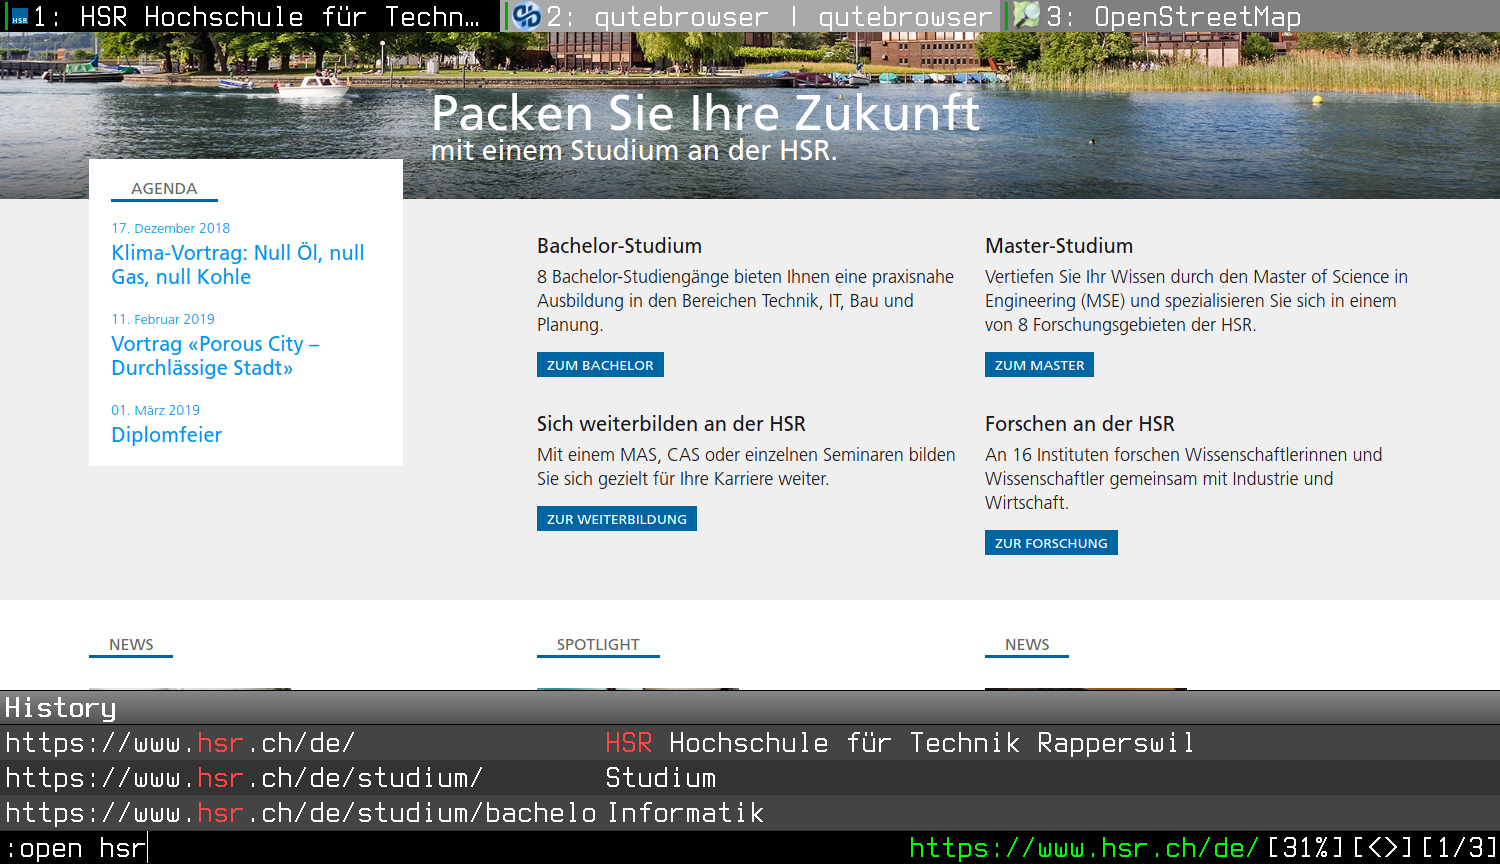
\includegraphics[width=\linewidth]{img/screenshot-intro.png}
\caption{qutebrowser displaying its history completion}
\end{figure}

\section*{Procedure / Results}
Before attempting to expose an interface for extensions from qutebrowser,
various problematic areas in qutebrowser's codebase had to be cleaned up due to
``technical debt'' accumulating in the past. Subsequently, functionality
suitable for moving out of the core into extensions was identified. Based on
the selected areas of code, a concept for an extension API\footnote{Application
programming interface} was developed. After implementing said API in
qutebrowser, large parts of functionality (such as the adblocker, blocking
advertisements on websites) could be moved into extensions. The resulting
changes increased code maintainability and simplicity.

In order to further follow best practices in the software development world,
tools for checking data types (thus reducing the chance of accidental software
defects) were evaluated. The \emph{mypy} tool is now run regularly over
qutebrowser's code, which resulted in various lingering defects being found in
qutebrowser itself and in related projects. Important parts of qutebrowser were
annotated with type information in order to find such issues, also serving as
additional developer documentation.

\section*{Future Work}
This research project was focused on increasing qutebrowser's software quality
and moving parts of its core into extensions. As a next step, additional
functionality should be exposed to extensions, allowing more code to be moved
out of the core.

When the exposed interfaces are expected to be reasonably stable,
they should then be gradually opened to interested external developers so that
third-party extensions can be written.

After third-party extensions gain enough traction, an ``extension manager''
should be developed, so that users can easily install and update available
extensions via a graphical interface.

\tableofcontents

\listoffigures
{\let\clearpage\relax \listoftables}
{\let\clearpage\relax \listoflistings}


% Aufgabenstellung
\chapter*{Task Definition}

% Einführung
\chapter{Introduction}
\label{ch:intro}

\section{Background}

The qutebrowser project is a web browser, comparable to Google Chrome or Mozilla
Firefox, which is focused on being keyboard-driven and having a minimal user
interface. It is aimed at power users who value customizability and efficiency,
but are willing to accept a rather steep learning curve compared to
``traditional'' web browsers.

Its philosophy and keybindings are inspired by the Vim
editor\footnote{\url{https://www.vim.org/}} which is available on almost any
UNIX system (such as macOS or Linux). Similar projects exist as addons for
Firefox (such as Tridactyl\footnote{\url{https://github.com/tridactyl/tridactyl}})
or Chrome (Vimium\footnote{\url{https://vimium.github.io/}}). However, due to
being constrained by the extension API exposed by Firefox and Chrome, those
projects lack various features which qutebrowser offers.

The project was started in December 2013 and is based on Python and PyQt5. An
extension API for users to write their own extensions to qutebrowser is a
long-standing feature
request\footnote{\url{https://github.com/qutebrowser/qutebrowser/issues/30}},
which has often been requested by its users.

It is difficult to estimate qutebrowser's user count, but it is most likely used by a
couple thousand users, so an extension API is also vital in order to be able to move
less popular features out of the core part of qutebrowser.

\fixme{Make clear that we're dealing with existing engines, maybe name, maybe motivation?}

\label{backends}
There are two backends (rendering engines) which can be used with qutebrowser:

\begin{itemize}
  \item \emph{QtWebKit} which is based on the
  WebKit\footnote{\url{https://www.webkit.org/}} project
  \item \emph{QtWebEngine} which is based on the
  Chromium\footnote{\url{https://www.chromium.org/}} project, which is also used
  in Google Chrome (used as default).
\end{itemize}

In order to allow using either backend, qutebrowser provides an abstraction
layer over the two libraries, implementing the adapter pattern
\autocite[139ff]{gof}. This abstraction layer is referred to as ``tab API'', and
documented in section \ref{tabapi}.

% Problemstellung, Vision
\section{Vision}
\label{vision}

Many qutebrowser users are power-users and, as such, have very specific (and
sometimes unique) feature requests and workflows. It should be possible for
those users to extend qutebrowser with custom extensions in an easy way, in order
to keep qutebrowser's core small.

Since qutebrowser already has a thriving community, this change also intends to
decentralize development efforts, as it enables users and developers to maintain
their extensions independently from the core development.

% Ziele und Unterziele
\section{Objectives}
\label{goals}

\subsection{Merging contributions}

\subsection{Refactorings}
\label{sec:goals-refactorings}

Initially, qutebrowser was developed without knowledge of proper software
engineering practices, which resulted in some maintainability issues. While many
of those issues have since been resolved, some still remain. Those
refactorings affect the API exposed to extensions, and therefore should be taken
care of before attempting to design a extension API.

The full list of relevant refactorings is tracked as a Kanban
board\footnote{\url{https://github.com/qutebrowser/qutebrowser/projects/3}} in
qutebrowser's GitHub repository. The biggest planned changes are the following:

\begin{itemize}
  \item \url{https://github.com/qutebrowser/qutebrowser/issues/1456}: \\ Parts of qutebrowser already use Python type
    annotations\footnote{\url{https://www.python.org/dev/peps/pep-0484/}}, but
    only if contributors decide to use them. In addition to that, no type
    checker such as mypy\footnote{\url{http://mypy-lang.org/}} is currently run
    as part of qutebrowser's continuous integration (CI) pipeline, thus allowing
    regressions to occur. As part of this project, a type checker should be
    introduced into the CI infrastructure, and any code exposed via the extension
    API should be annotated with proper type annotations.
  \item \url{https://github.com/qutebrowser/qutebrowser/issues/345}: \\
    To generate HTML documentation, qutebrowser currently uses
    asciidoc\footnote{\url{http://asciidoc.org/}} which is unsuitable for API
    documentation and ceased maintenance. An external contributor (see page
    \pageref{fiete}) is currently working on migrating to the
    Sphinx\footnote{\url{http://www.sphinx-doc.org/}} toolchain, and should be
    supported with his work throughout the SA. \fixme{update}
  \item \url{https://github.com/qutebrowser/qutebrowser/issues/640}: \\
    Global objects are registered in a object registry based on a name as
    string (``stringly-typed''\footnote{\url{http://wiki.c2.com/?StringlyTyped}}).
    This historically caused various object-lifetime related issues, and also
breaks tooling such as the mypy type checker. All code using the object registry
should be refactored to use better alternatives such as constructor arguments
(dependency injection).
\end{itemize}

\subsection{Extension API}

\subsection{Documentation}

\fixme{continue!}

% Rahmenbedingungen, Umfeld, Definitionen, Abgrenzungen
\section{Context}
\label{context}

The software and version constraints are mostly given by the existing project:

\begin{itemize}[parsep=5pt]
  \item Python\footnote{\url{https://www.python.org/}} 3 (3.5 or newer)
  \item Qt\footnote{\url{https://www.qt.io/}} 5 (5.7 or newer), used via PyQt5\footnote{\url{https://www.riverbankcomputing.com/software/pyqt/intro}}
  \item pytest\footnote{\url{https://pytest.org/}} as test framework
  \item Various code quality tools: pylint\footnote{\url{https://pylint.org/}},
    flake8\footnote{\url{http://flake8.pycqa.org/}} and others.
\end{itemize}

As qutebrowser is a pre-existing project with a vibrant community, external
contributions are expected to continue (despite an
announcement\footnote{\url{https://lists.schokokeks.org/pipermail/qutebrowser-announce/2018-October/000053.html}, accessed 2018-11-12}
asking people to refrain from making larger contributions). This can be challenging,
as it results in refactorings being carried out against a moving target. Because
of the nature of open-source contributions,
% http://www.catb.org/~esr/writings/cathedral-bazaar/cathedral-bazaar/
% https://www.fordfoundation.org/about/library/reports-and-studies/roads-and-bridges-the-unseen-labor-behind-our-digital-infrastructure/
it is hard to foresee or control which areas external contributors are changing.
At the beginning of the SA, some time was allocated for merging external
contributions (pull requests) which were already open. For the rest of the SA,
such contributions will be dealt with on a best effort basis, with the main
focus being this documentation and the work required for the extension API.

\fixme{Describe Python decorators, packages/modules, Qt signals/slots}

% Vorgehen, Aufbau der Arbeit
\section{Methods and Structure}
\subsection{Structure of this document}
This document is organized in roughly chronological order.

In this chapter, the background necessary to understand the
project and its goals is explained. Chapter \ref{ch:projectman} documents the
project methodology used and allocates the time available.
It also analyzes the risks involved. Chapter \ref{ch:requirements} specifies the
project requirements in more detail. In chapter \ref{ch:existing}, existing
similar work is examined. Chapter \ref{ch:evaluation} notes the criteria being
considered for the project. Based on those criteria, a concept was designed in chapter
\ref{ch:concept}. Finally, chapter \ref{ch:implementation} explains the actual
implementation, while chapter \ref{ch:results} analyzes the results.

In appendix \ref{ch:glossary}, a glossary of the terms and abbreviations used
can be found.

\subsection{Design decisions}
\fixme{How to cite y-approach? - cite SATURN presentation instead}

In order to take informed and sustainable design decisions, the
\emph{Y-Approach} \autocite{yapproach} was evaluated. It proposes the following
template for design decisions:

\begin{quote}
  \begin{itemize}[parsep=5pt]
    \item In the context of \emph{use case $uc$ and/or component $co$},
    \item \ldots facing \emph{non-functional concern $c$},
    \item \ldots we decided for \emph{option $o_1$}
    \item and neglected \emph{options $o_2$ to $o_n$},
    \item \ldots to achieve \emph{quality $q$},
    \item \ldots accepting downside \emph{consequence $c$}.
  \end{itemize}
\end{quote}

The template serves as a good reminder of the aspects to keep in mind
while taking a decision. However, it was found to not be very helpful for
documentation, as a different structure (such as a list of considerations, or
prose text) is often more readable. Thus, it was used as an inspiration only,
but the explanations in this document do not strictly follow its structure.

\fixme{we don't need high-level decisions}

\subsection{Tools used}
Since this project was realized by a single author (rather than in a group),
project management tooling was kept to a minimum. GitHub issues and its project
board features were used for project management, along with
Clockify\footnote{\url{https://www.clockify.me/}} for time tracking.

This document was typeset in \LaTeX{} using the \emph{Computer Modern Bright}
font and various additional packages. GNU Emacs was used as text editor.

% Projektmanagement (Planung, Soll)
\chapter{Project Management}
\label{ch:projectman}

% Prototypen, Releases, Meilensteine
\section{Prototypes, Releases, Milestones}
Since this project is done without any external industry partner, there is no
immediate need for fixed releases or prototypes during the SA.

However, the following releases are planned:

\begin{itemize}
  \item A v1.5.0 feature release as soon as PyQt 5.11.3 is released upstream
    \begin{itemize}
      \item v1.5.0 was released in week 3
    \end{itemize}
  \item Patch releases for v1.5.x as needed in case of regressions or serious
    enough bugs:
    \begin{itemize}
      \item v1.5.1 was released in week 4
      \item v1.5.2 in week 6
      \item v1.5.3 in week \fixme{}
    \end{itemize}
  \item v1.6.0 after the work on refactoring qutebrowser's core into extensions
    is completed, in order to get the changes out to users as soon as possible.
  \item v1.6.x patch releases as needed (probably after the SA is finished)
  \item In the future, after the extension API is open for third-party
    extensions, a v2.0.0 release with some other big changes (like dropping support
    for the older QtWebKit backend, as it's rarely updated upstream, even for
    security issues).
\end{itemize}

At the end of week 11, an API review milestone is planned, where the extension
API design gets reviewed by employees of the IFS (Institute for Software) at the
HSR.

% Team, Rollen und Verantwortlichkeiten
\section{Team and Roles}
\emph{Florian Bruhin} is both the primary maintainer of qutebrowser and the
sole author of this student research project. He has been working on qutebrowser since
December 2013 and started studying Computer Science at HSR in 2016.

\emph{Joël Schwab} intended to co-author this research project, but
unfortunately didn't pass some exams, which were a precondition to be allowed to
do the SA project this semester.

Professor \emph{Stefan Keller}, institute partner at the Institute for Software
(IFS) at HSR is the advisor for this project.

\emph{Raphael Das Gupta}, research assistant at the IFS, helped out with code
reviews and architectural decisions.

The qutebrowser community is not directly involved in this research project, but
is the primary audience of the resulting work. It has also contributed many
ideas and use cases for future
extensions\footnote{\url{https://github.com/qutebrowser/qutebrowser/issues/30}}.
There is no external industry partner.

\label{fiete}
\emph{Fritz Reichwald} (fiete201\footnote{\url{https://github.com/fiete201}})
is a long-time qutebrowser user who is working on migrating qutebrowser's
documentation system from asciidoc\footnote{\url{http://asciidoc.org/}} (which
is deprecated) to the Sphinx\footnote{\url{http://www.sphinx-doc.org/}}
documentation generator. This change was
planned\footnote{\url{https://github.com/qutebrowser/qutebrowser/issues/345}}
since December 2014, so his help with tackling this is very much appreciated.
This project will benefit from his work, as Sphinx, unlike asciidoc, is a
very good fit for documenting APIs. His work is clearly marked as such in this
documentation. \fixme{update}

% Prozessmodel
\section{Process Model}
Because of previous experience as part of HSR's ``Engineering Project'', the
``Scrum+'' process model will be used, i.e., an agile Scrum process with an
additional ``End of Elaboration'' milestone.

At the beginning of the SA, there was a phase with the goal of merging existing
third-party contributions (pull requests) into qutebrowser, so that the changes
required for extensions does not conflict with existing work. Thus, an additional
\emph{preparation} phase has been introduced, resulting in the following phases:

Inception, Preparation, Elaboration, Construction, Transition

% Aufwandschätzung, Zeitplan, Projektplan
\section{Project Schedule}
\label{schedule}

8 ECTS credits are awarded for the SA-course. Since one ECTS point is equivalent
to a workload of 25--30 hours \autocite{ects} and this SA is written by a single
author, this amounts to 200--240 hours of work. The semester consists of 14
weeks, thus, an average workload of 14--17 hours per week is expected. This time
is allotted as shown in figure \ref{img:schedule}.

\begin{figure}[h!]
  \begin{ganttchart}[
        title height = 1,
        y unit title=.5cm,
        y unit chart=.5cm,
        bar/.append style={fill=green!20},
        vgrid={
          *1{blue!60},
          *4{gray, dashed},
          *1{blue!60},
          *2{gray, dashed},
          *1{blue!60},
          *2{gray, dashed},
          *1{gray, dashed}
        }]{1}{14}
    \gantttitle{\hspace{-6.5em}\footnotesize{Calendar week}}{0}{0}
    \gantttitlelist{38,...,51}{1} \\
    \gantttitle{\hspace{-6.5em}\footnotesize{Semester week}}{0}{0}
    \gantttitlelist{1,...,14}{1} \\

    \ganttgroup{Inception}{1}{1} \\
    \ganttmilestone{M0: Kickoff}{1} \\

    \ganttgroup{Preparation}{2}{6} \\
    \ganttbar{Qt 5.12 release}{2}{2} \\
    \ganttbar{Merge contributions}{3}{5} \\
    \ganttbar{Buffer}{6}{6} \\

    \ganttmilestone{M1: Most contributions addressed}{6} \\

    \ganttgroup{Elaboration}{7}{9} \\
    \ganttbar{Existing approaches}{7}{7} \\
    \ganttbar{Project documentation}{8}{8} \\
    \ganttbar{API design}{9}{9} \\

    \ganttgroup{Construction}{10}{13} \\
    \ganttbar{Introducing MyPy}{10}{10} \\
    \ganttbar{Adding extension API}{11}{12} \\
    \ganttmilestone{M2: API review}{11} \\
    \ganttbar{Refactoring core into extensions}{11}{12} \\
    \ganttmilestone{M3: v1.6.0 release}{12} \\
    \ganttbar{Buffer}{13}{13} \\

    \ganttgroup{Transition}{14}{14} \\
    \ganttbar{Finishing documentation}{14}{14} \\

    \ganttmilestone{M4: Project end}{14}
  \end{ganttchart}
  \caption{Project schedule}
  \label{img:schedule}
\end{figure}

\fixme{feature freeze}

Due to the relatively long \emph{preparation} phase at the beginning of the
project, the \emph{construction} phase gets unusually short. This is
unfortunate but unavoidable -- it's important to integrate existing
contributions before starting to refactor the existing code, at least for
third-party changes which would lead to conflicts with refactoring changes.

% Risiken
\section{Risks}
\label{sec:risks}
The following risks have been identified in this project:

\fixme{Should have a time, if possible -- see ÖV-Güteklassen 2018?}

\begin{table}[h!]
  \begin{tabulary}{\linewidth}{LLL}
    \toprule
    Risk & Mitigation & Probability (1-5) \\
    \midrule
    Too many external contributions & Asking contributors to hold back further contributions; ignoring existing contributions & 5 \\
    \hline
    Little time in construction phase & Work on extension API is very
    scalable, buffers in schedule & 4 \\
    \hline
    Sickness of author & Work on extension API is very scalable & 3 \\
    \hline
    Future breaking API changes needed & API is not exposed for third-party
    contributions yet & 3 \\
    \hline
    Migrating documentation toolchain to Sphinx (done by external contributor)
    is not done in time \fixme{update }& Initial extension API documentation can be separate from
    qutebrowser documentation & 3 \\
    \bottomrule
  \end{tabulary}
\end{table}

As explained in section \ref{context}, it's expected that third-party
contributors continue to submit changes (in the form of pull requests) while
this SA is ongoing. An
announcement\footnote{\url{https://lists.schokokeks.org/pipermail/qutebrowser-announce/2018-October/000053.html},
  accessed 2018-11-12} was sent out, asking contributors to cut back external
contributions. However, a similar announcement was sent out during past exam
seasons, with mixed results -- many contributors continue to submit changes
regardless. Initially, there's a phase focused on merging existing
contributions (see the project schedule in section \ref{schedule}). Afterwards,
contributions are dealt with on a best effort basis, being ignored if they
are non-trivial.

There's little time in the construction phase compared to other projects.
Additionally, this SA is written by a single author. Thus, sickness or other
obstructions have a bigger than usual impact. This is counteracted by trying to
keep the scope of the SA clear, but flexible. Additionally, buffer time is
added after the preparation and construction phases in the project schedule
(section \ref{schedule}).

If some preparatory work isn't finished fully, it's possible that upcoming
changes cause incompatible changes in the extension API. However, this SA
is focused on moving core code into extensions, rather than providing an
extension API for third-party extensions. Therefore, it's still possible to make
those changes after the SA is finished, without breaking third-party code.


\chapter{Requirements Specification}
\label{ch:requirements}

% Use Cases (Success Scenario / Success Diagram)
\section{Use Cases}

This project extends an existing codebase with an extension API rather
than starting a new project from scratch. By its nature, it's difficult to
predict how an extension API will be used in the future. Because of that, an
use-case diagram would not adequately describe the motivation for the extension
API.

Various ideas for future third-party extensions have been voiced by the
qutebrowser community; they are collected in a GitHub
issue\footnote{\url{https://github.com/qutebrowser/qutebrowser/issues/30},
  accessed 2018-11-08}. However, the main aim of this project (and thus the main
focus for the extension API) is reducing the complexity of qutebrowser's core.

% Weitere Funktionen, die nicht erfasst wurden
%\section{Further Functionality}

% Nicht-funktionale Anforderungen (Rahmbenbedingungen, evtl. Verweis auf 1.3)
\section{Non-functional Requirements}
The following non-functional requirements are relevant for qutebrowser's
extension API:

\begin{description}
  \item[Security] The security model used for qutebrowser extensions assumes
    that extensions are trusted, i.e., may run arbitrary code. See
    section \ref{security} for a more detailed explanation.
  \item[Simplicity] It should be trivial for a user to extend her qutebrowser
    setup with a custom extension. Thus, getting started with writing a
    third-party extension should be as straightforward as possible, without
    requiring packing multiple files into a custom format. Also see section
    \ref{anatomy} for an explanation on how this topic is handled for
    WebExtensions, and how qutebrowser's API differs from that.
  \item[Learnability] When the extension API is opened for third-party
    contributions, it should be easy to get accustomed to it. Therefore, the API
    should be intuitive for Python programmers, and well documented.
  \item[Compability] The qutebrowser project runs on a variety of different
    software versions -- various operating systems (Linux, macOS, Windows,
    and more) are supported, including different Qt and Python versions. The
    extension API should abstract over those differences, so an extension
    written for qutebrowser (or core code moved into such an extension) runs in
    all situations qutebrowser itself can run.
  \item[Performance] Having code in extensions (rather than in the core part of a
    project) can result in performance degradations due to more moving parts and
    more layers being involved. Since those impacts are usually small
    individually (but might be big enough to be relevant collectively), no
    relevant impact is expected in the scope of this SA. However, performance
    considerations might be a good reason to keep some code in the core rather
    than moving it to extensions in the future.
\end{description}

% % Detailspezifikation
% \section{Detailed Specification}
% \fixme{???}
% 
% % Analyse (Business Model)
% \chapter{Analysis}
% 
% % Domain Modell, Klassendiagramme (konzeptionell)
% \section{Domain Model}
% 
% % Objektkatalog (Beschreibung der Konzepte, bzw. Entitätsmengen)
% \section{Objects}

% "Stand der Technik" (Was gibt es schon?)
\chapter{Existing APIs}
\label{ch:existing}
\label{unsuitable}

Other browsers (such as Firefox or Chrome) have been supporting extensions for a
long time. When designing an extension API, it is useful to understand this
previous work. It can serve as an inspiration, in order to follow common standards and learn
from mistakes made in the past. Therefore, various existing extension APIs have
been analyzed.

\section{Firefox XUL extension API}

Older versions of the Firefox web browser used to have a very powerful extension
API, based on its XUL (XML User Interface Language) technology. However, this
approach presented various challenges and was thus recently abandoned, while
adopting the WebExtensions standard.

The apparent philosophy behind ``legacy'' Firefox addons was to allow maximum
customizability from extensions -- however, this came with various drawbacks
which ultimately led to Mozilla abandoning that approach.

The motivations to deprecate and subsequently remove the legacy addon API listed
in Mozilla's blog post \autocite{mozilla-webext} were as follows:

\begin{itemize}
  \item Chrome and Opera (and nowadays also Microsoft Edge) already supported
    the WebExtension API, so a switch to the WebExtension API would drastically
    reduce the effort required for developers when implementing extensions with
    cross-browser compatibility: \emph{``We would like add-on development to be more
    like Web development: the same code should run in multiple browsers according to
    behavior set by standards, with comprehensive documentation available from
    multiple vendors.''}
  \item Firefox' Electrolysis (e10s)
    project\footnote{\url{https://wiki.mozilla.org/Electrolysis}} was a big
    change in its codebase, with the goal of separating tabs into separate
    processes, for security and performance reasons. Many legacy addons were not
    compatible with the changes necessary for Electrolysis. This forced either
    the add-on developer to make (sometimes intricate) changes to their code; or
    the user's Firefox instance to run in a special fallback mode: \emph{``Add-ons
    that haven't been upgraded to work with Electrolysis will run in a special
    compatibility environment that resembles single-process Firefox as much as
    possible. [...] However, [the fallback is] much slower than the equivalent DOM
    operations in single-process Firefox, and can affect the user experience
    negatively. Also, some accesses aren't supported by the compatibility layer and
    will throw exceptions.''}
  \item Since Firefox is a quite popular product, malicious Firefox addons
    started to become an attractive attack vector for bad actors. With legacy
    addons, addon code is able to run arbitrary code and freely modify Firefox
    internals on the user's machine, which turns untrusted addons into a
    security liability \autocite{mozilla-signing}.
  \item Legacy addons hindered Firefox development in general, since its
    powerful addon API introduced a tight coupling between Firefox' internal
    code, and the code in third-party addons: \emph{``A permissive add-on model
    means that we have limited flexibility in changing the foundations of Firefox.
    [...] Without a fundamental shift to the way Firefox add-ons work, we will
    be unable to use new technologies like Electrolysis, Servo\footnote{An
      experimental new rendering engine by Mozilla, implemented in the Rust
      programming language. Parts of Servo (such as its CSS renderer) have since
    been merged into Firefox.} or browser.html\footnote{A Mozilla research
    project which implements a browser completely in HTML, now retired.}
    as part of Firefox. The tight coupling between the browser and its add-ons
    also creates shorter-term problems for Firefox development. It's not uncommon
    for Firefox development to be delayed because of broken add-ons.''}
\end{itemize}

While qutebrowser should learn from the mistakes made in Firefox' legacy API,
a more thorough analysis of the XUL API design proved to be difficult. Archived
API documentation is still
available\footnote{\url{https://developer.mozilla.org/en-US/docs/Archive/Add-ons}},
but bad documentation was one of the criticisms of XUL addons
\autocite{mozilla-webext}. Since the API is not in active use anymore, and ties
into Firefox' core code deeply, no further analysis was performed.

The key takeaway for qutebrowser is that it should have a minimal and clearly
outlined extension API, rather than naively exposing its internal Python code to
extensions.

\section{WebExtensions API}
\label{webextensions}

Currently, there are ongoing efforts towards an API for browser
extensions called \emph{WebExtensions}, which is shared between different
browsers. WebExtensions are supported by Chrome, Opera, Firefox and Edge.
Efforts are currently underway to standardize the API as a W3C specification
\autocite{w3c-webext}. At the moment, each browser has a slightly different set of
supported APIs, with some divergence in naming. As an example, the
\verb|chrome.| module is used in Chromium for browser-specific features, while
Firefox uses \verb|browser.|.

If qutebrowser supported the WebExtension API, it would follow a common
standard, and enable running thousands of existing Chromium extensions with
little to no adjustment to their code.

Unfortunately, WebExtensions are unsuitable for qutebrowser, for various
reasons:

\begin{itemize}
  \item Full WebExtension support would likely require some degree of support by
    the underlying rendering engine. While there is an open
    suggestion\footnote{\url{https://bugreports.qt.io/browse/QTBUG-61676}} in
    Qt's bug tracker, no work on that has been started so far.
  \item Implementing WebExtension support in Python only (without any support
    from the underlying backend) is hard, if possible at all. Neither
    backend allows deep access to its JavaScript engine
    (V8\footnote{\url{https://v8.dev/}} for QtWebEngine, JavaScriptCore for
    QtWebKit), which means extension code would have to run in a separate
    JavaScript interpreter (such as Qt's
    \verb|QJSEngine|\footnote{\url{http://doc.qt.io/qt-5/qjsengine.html}} class).
    However, extensions should have access to web contents. Thus, a secure
    communication channel is needed between the backend's JavaScript interpreter
    (used for the page), and the separate interpreter used for extensions. In
    addition, it should only be possible for extensions to access page content,
    not the other way around, as that would be a security issue. All in all,
    this approach is prohibitively complex, and thus out of scope for this SA.
  \item Most qutebrowser users and contributors are accustomed to writing Python
    code (since qutebrowser itself is written in Python). While a WebExtension
    API (in JavaScript) would allow using thousands of existing Chrome extensions, a
    Python API will make it easier for users to write custom additions to
    qutebrowser to suit their needs.
  \item The security model of WebExtensions is fundamentally different from
    what's intended for qutebrowser extensions -- WebExtension code is sandboxed,
    and unable to run arbitrary code on the user's machine. This can be worked
around by using WebExtension's ``native
    messaging''\footnote{\url{https://developer.mozilla.org/en-US/docs/Mozilla/Add-ons/WebExtensions/Native_messaging}}
    capability with a separate application running in the background, but doing
    so is cumbersome. See \ref{security} for an explanation on the security
    model of qutebrowser extensions.
  \item The WebExtension API was not designed with the Qt APIs in mind, yet
    qutebrowser is bound to using those. In some cases it might be possible to
    write an adapter to bring the two approaches together; but if they are
    fundamentally different, doing so might prove difficult. With a custom API,
    there's more control over the tradeoff between an API which closely follows
    Qt's (and thus reduces friction and complexity), or an API which prioritizes
    other considerations (see \ref{criteria}).
\end{itemize}

While it is not possible for qutebrowser to implement support for WebExtensions,
they are still useful as a source for API design inspiration. However, it
should be noted that the WebExtension API is closely tied to the JavaScript
language, so architecture decisions taken there will not necessarily be
applicable to qutebrowser's Python extension API.

\subsection{Anatomy of a WebExtension}
\label{anatomy}

As explained in Mozilla's
documentation\footnote{\url{https://developer.mozilla.org/en-US/docs/Mozilla/Add-ons/WebExtensions/Anatomy_of_a_WebExtension},
  accessed 2018-11-08},
a WebExtension consists of various files:

\begin{itemize}
  \item A \verb|manifest.json| manifest file, which lists meta information about
    an extension, such as its name, its author, or the permissions it requests.
  \item Background scripts, which are used to implement long-running operations.
    An extension's background scripts are loaded for the entire lifetime of an
    extension, i.e., until it is disabled or uninstalled.
  \item Content scripts, which are injected into loaded web pages, and can
    interact with their content (access and manipulate the DOM). They also have
    some additional permissions, which scripts supplied by the page do not have,
    such as messaging with an extension's background scripts.
  \item HTML pages for user interfaces such as an extension's option page or sidebar.
  \item Other resources such as icons.
\end{itemize}

Those files are then packaged into a specially named ZIP file (XPI in case of
Firefox; CRX for Chromium) and distributed via an extension store (a special
website run by Mozilla/Google).

For qutebrowser extensions, a simpler approach will be taken: Extensions can
consist of a single standalone \verb|.py| file which implements the necessary
functionality. This mechanism is inspired by the plugin handling of the pytest
project\footnote{\url{https://docs.pytest.org/en/latest/writing_plugins.html},
  accessed 2018-11-08}. In the future, this makes it trivial for users to add
their own extensions to qutebrowser. That solution is also very straightforward and
appropriate for the initial goal of refactoring qutebrowser's core code into
extensions.

Due to extensions being written in Python, the above separation between content
and background scripts also does not fully apply to qutebrowser's API. The Python
extensions can be seen as a background script. It initially won't be able to
interact with web pages, as this functionality isn't needed before third-party
extensions are enabled. See the API analysis below for further details.

\subsection{Analysis of the WebExtension API}

The WebExtensions API is separated into various modules, each of which is
briefly analyzed in the context of qutebrowser in this section, sorted
alphabetically. The indented descriptions are copied verbatim from Mozilla's API
documentation\footnote{\url{https://developer.mozilla.org/en-US/docs/Mozilla/Add-ons/WebExtensions/API},
  \\ accessed 2018-11-02}.

\subsubsection{alarms}
\begin{quote}
Schedule code to run at a specific time in the future.
\end{quote}

Since qutebrowser extensions will have access to the Qt GUI library, no
equivalent to this module is needed. Qt provides the
\verb|QTimer|\footnote{\url{http://doc.qt.io/qt-5/qtimer.html}} class, which can
be used for equivalent functionality.

\subsubsection{bookmarks}
\begin{quote}
The WebExtensions bookmarks API lets an extension interact with and manipulate the browser's bookmarking system. You can use it to bookmark pages, retrieve existing bookmarks, and edit, remove, and organize bookmarks.
\end{quote}

Bookmarks in qutebrowser are currently much simpler than they are in Firefox or
Chrome; i.e. they are not organized in a tree-like structure, and features like
tags are missing. Therefore, the bookmarks WebExtension API does not fit well
with qutebrowser bookmarks.

There's an ongoing
contribution\footnote{\url{https://github.com/qutebrowser/qutebrowser/pull/3855}}
to add such features, and it would make little sense to add an extension API before
that contribution is merged. Since access to bookmarks isn't vital for an extension
API, it is currently out of scope.

\subsubsection{browserAction, menus, pageAction, sidebarAction}
\begin{quote}
browserAction: Adds a button to the browser's toolbar.
\end{quote}
\begin{quote}
menus: Add items to the browser's menu system.
\end{quote}
\begin{quote}
pageAction: A page action is a clickable icon inside the browser's address bar.
\end{quote}
\begin{quote}
sidebarAction: Gets and sets properties of an extension's sidebar.
\end{quote}

Those modules allow extensions to add their own user interface elements to the
browser, as shown in figure \ref{img:browser-action}.

\begin{figure}[h]
  \centering
  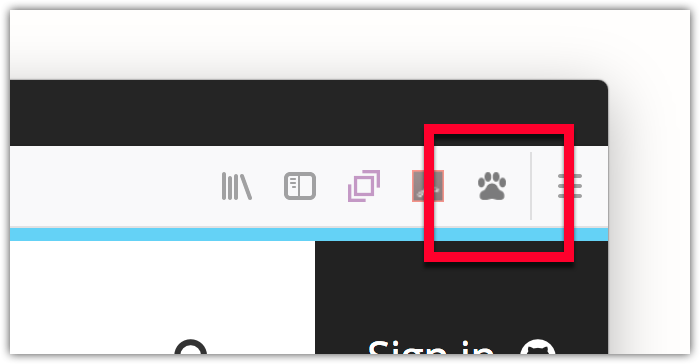
\includegraphics[width=0.5\linewidth]{img/browser-action.png}
  \caption{A button added via the \texttt{browserAction} WebExtension API}
  \label{img:browser-action}
\end{figure}

It should be possible for custom qutebrowser extensions to add their own user
interface elements. However, this functionality is unlikely to be needed
when moving core functionality into extensions (which is the main focus of this
SA). Therefore, this API is currently out of scope.

\subsubsection{browserSettings}
\begin{quote}
Enables an extension to modify certain global browser settings.
\end{quote}

Extensions for qutebrowser should be able to modify its settings, and also
define their own options.

\subsubsection{browsingData}
\begin{quote}
Enables extensions to clear the data that is accumulated while the user is
browsing.
\end{quote}

No such functionality is currently implemented in qutebrowser, so this API is
out of scope.

\subsubsection{clipboard}
\begin{quote}
The clipboard API enables an extension to copy items to the system clipboard.
\end{quote}

Since qutebrowser extensions will have access to the Qt GUI library, no
equivalent to this module is needed. Qt provides the
\verb|QClipboard|\footnote{\url{http://doc.qt.io/qt-5/qclipboard.html}} class, which can
be used for equivalent functionality.

\subsubsection{commands}
\begin{quote}
Listen for the user executing commands that you have registered using the commands manifest.json key.
\end{quote}

This API is used to register custom keyboard shortcuts in WebExtensions. A
similar concept also exists in qutebrowser, where commands can either be bound
to keys (using the configuration), or executed in the commandline via \verb|:command|.

This API is important, since many core parts register commands in qutebrowser
(like \verb|:adblock-update| for the ad blocker). Thus, Extensions should be
able to register Python functions as commands.

\subsubsection{contentScripts}
\begin{quote}
With the contentScripts API, an extension can register and unregister scripts at runtime.
\end{quote}

Injecting custom JavaScript code into websites will be an useful feature for
custom extensions at a later stage, but isn't needed to move code out of
qutebrowser's core, as it's expected for internal JavaScript code to stay in the
core part. Thus, this module is currently out of scope.

Running JavaScript one-off snippets (triggered manually, rather than
automatically on page load) is already implemented in the tab API, and should be
trivial to expose to extensions.

\subsubsection{contextualIdentities, i18n, identity, idle, notifications, pkcs11, topSites}
\begin{quote}
contextualidentities: Work with contextual identities: list, create, remove, and update contextual identities.
\end{quote}
\begin{quote}
i18n: Functions to internationalize your extension. You can use these APIs to get localized strings from locale files packaged with your extension, find out the browser's current language, and find out the value of its Accept-Language header.
\end{quote}
\begin{quote}
identity: Use the identity API to get an OAuth2 authorization code or access token, which an extension can then use to access user data from a service which supports OAuth2 access (such as a Google or a Facebook account).
\end{quote}
\begin{quote}
idle: Find out when the user's system is idle, locked, or active.
\end{quote}
\begin{quote}
notifications: Display notifications to the user, using the underlying operating system's notification mechanism.
\end{quote}
\begin{quote}
pkcs11: The pkcs11 API enables an extension to enumerate PKCS\#11 security modules, and to make them accessible to the browser as sources of keys and certificates.
\end{quote}
\begin{quote}
topSites: Use the topSites API to get an array containing pages that the user has visited often and frequently.
\end{quote}

No such functionality is currently implemented in qutebrowser, so those modules
are out of scope.

\subsubsection{cookies}
\begin{quote}
Enables extensions to get and set cookies, and be notified when they change.
\end{quote}

Cookie access isn't fully exposed by the QtWebEngine
library\footnote{\url{http://doc.qt.io/qt-5/qwebenginecookiestore.html}}, so
it's currently not possible to implement this module.

\subsubsection{devtools}
\begin{quote}
The devtools.inspectedWindow API lets a devtools extension interact with the window that the developer tools are attached to.
\end{quote}

\begin{quote}
The devtools.network API lets a devtools extension get information about network requests associated with the window that the devtools are attached to (the inspected window).
\end{quote}

\begin{quote}
The devtools.panels API lets a devtools extension define its user interface inside the devtools window.
\end{quote}

Access to developer tools isn't exposed by the QtWebEngine library, so it's
currently not possible to implement this module.

\subsubsection{dns}
\begin{quote}
Enables an extension to resolve domain names.
\end{quote}

Since qutebrowser extensions will have access to the Qt GUI library, no
equivalent to this module is needed. Qt provides the
\verb|QDnsLookup|\footnote{\url{http://doc.qt.io/qt-5/qdnslookup.html}} class, which can
be used for equivalent functionality.

\subsubsection{downloads}
\begin{quote}
Enables extensions to interact with the browser's download manager. You can use this API module to download files, cancel, pause, resume downloads, and show downloaded files in the file manager.
\end{quote}

This module is needed for various core parts (such as the ad blocker, to
download filter lists).

\subsubsection{events, extensions, extensionTypes, permissions, runtime, types}
\begin{quote}
events: Common types used by APIs that dispatch events.
\end{quote}
\begin{quote}
extensions: Utilities related to your extension. Get URLs to resources packages with your extension, get the Window object for your extension's pages, get the values for various settings. Note that the messaging APIs in this module are deprecated in favor of the equivalent APIs in the runtime module.
\end{quote}
\begin{quote}
extensionTypes: Some common types used in other WebExtension APIs.
\end{quote}
\begin{quote}
permissions: Extensions need permissions to access more powerful WebExtension APIs. They can ask for permissions at install time, by including the permissions they need in the permissions manifest.json key. The main advantages of asking for permissions at install time are:
\end{quote}
\begin{quote}
runtime: This module provides information about your extension and the environment it's running in.
\end{quote}
\begin{quote}
types: Defines the BrowserSetting type, which is used to represent a browser setting.
\end{quote}

Those APIs are specific to the WebExtensions API, and thus irrelevant for
qutebrowser.

\subsubsection{find}
\begin{quote}
Finds text in a web page, and highlights matches.
\end{quote}

This functionality is already available as part of qutebrowser's tab API (see
section \ref{tabapi}), and should be trivial to expose to extensions.

\subsubsection{history}
\begin{quote}
Use the history API to interact with the browser history.
\end{quote}

Accessing and manipulating the history might be an useful feature for future
user-contributed extensions, but is likely not needed for moving code out of
qutebrowser's core. Thus, the history module is currently out of scope.

\subsubsection{management}
\begin{quote}
Get information about installed add-ons.
\end{quote}

Extensions are currently not expected to interact with each other (even less so
when moving code out of the core), so this module is not needed.

\subsubsection{omnibox}
\begin{quote}
Enables extensions to implement customised behavior when the user types into the
browser's address bar.
\end{quote}

When adding custom commands, extensions also should be able to specify a
completion function, so users can use qutebrowser's autocompletion when typing
the extension's commands.

\subsubsection{privacy}
\begin{quote}
Access and modify various privacy-related browser settings.
\end{quote}

In qutebrowser, those settings (like
\verb|privacy.network.webRTCIPHandlingPolicy|) are exposed as normal qutebrowser
setttings (like \verb|content.webrtc_ip_handling_policy|), so there's no need
for a similar module in the extension API.

\subsubsection{proxy}
\begin{quote}
Use the proxy API to proxy web requests. There are two different ways you can do this:
\end{quote}

No low-level networking access is possible via the QtWebEngine API, so this
module will not be implemented.

\subsubsection{search}
\begin{quote}
Retrieves search engines and executes a search with a specific search engine.
\end{quote}

Search engines are part of the main configuration in qutebrowser, so an
extension can trivially retrieve a search engine from there and execute a query
without the need for a dedicated API.

\subsubsection{sessions}
\begin{quote}
Use the sessions API to list, and restore, tabs and windows that have been closed while the browser has been running.
\end{quote}

While qutebrowser does have a session feature, access to it is not vital for an
extension API, so this is currently out of scope.

\subsubsection{storage}
\begin{quote}
Enables extensions to store and retrieve data, and listen for changes to stored items.
\end{quote}

Having a simple way to persist data for extensions will be an useful feature for
third-party extensions, but is currently not needed when moving code out of the core.

\subsubsection{tabs, windows}
\begin{quote}
tabs: Interact with the browser's tab system.
\end{quote}
\begin{quote}
windows: Interact with browser windows. You can use this API to get information about open windows and to open, modify, and close windows. You can also listen for window open, close, and activate events.
\end{quote}

Various functionality already exists in qutebrowser as part of the ``tab API''
(documented in section \ref{tabapi}), which should be trivial to expose to the
extension API. Furthermore, the \verb|tabs| and \verb|windows| modules contains
various functionality to retrieve tabs, which should be added to qutebrowser's
extension API.

\subsubsection{theme}
\begin{quote}
Enables browser extensions to update the browser theme.
\end{quote}

No dedicated theme feature exists in qutebrowser - instead, qutebrowser's user
interface can be customized using its configuration.

\subsubsection{webNavigation}
\begin{quote}
Add event listeners for the various stages of a navigation. A navigation consists of a frame in the browser transitioning from one URL to another, usually (but not always) in response to a user action like clicking a link or entering a URL in the location bar.
\end{quote}

This exposes various events such as \verb|webNavigation.onCompleted|. Those will
be exposed as part of the tab API in qutebrowser, as Qt signals such as \verb|load_finished|.

\subsubsection{webRequest}
\begin{quote}
Add event listeners for the various stages of making an HTTP request. The event listener receives detailed information about the request, and can modify or cancel the request.
\end{quote}

The \verb|webRequest| module allows extensions to intercept and change HTTP
network requests. Many of the fine-grained modifications exposed by
WebExtensions (such as \verb|onResponseStarted| to modify the network response)
are not available in the QtWebEngine API, so exposing them in qutebrowser's API
won't be possible. However, it's possible to intercept and block network
requests, and such functionality is critical to move components like the ad
blocker out from the core.

\section{qutebrowser tab API}
\label{tabapi}

As explained in section \ref{backends}, qutebrowser supports two rendering
engines (QtWebKit and QtWebEngine) and provides an abstraction layer (``tab
API'') over those backends, representing a single tab in the browser.

The tab API has been designed with clean API design in mind, as an extension API
already was on the horizon when implementing it. Its goal is that the rest of
qutebrowser's code never has to access backend-specific functionality (like the
\verb|QWebEngineView|\footnote{\url{https://doc.qt.io/qt-5/qwebengineview.html}}
class) directly, and uses the abstraction layer instead.

The tab API is grouped into various classes:

\begin{figure}[h]
\begin{tikzpicture}
  \begin{class}[text width=2cm]{Tab}{6,2}
  \end{class}

  \begin{class}[text width=2cm]{Audio}{0,0}
  \end{class}
  \mycomposition{Tab}{}{}{Audio}{}{}

  \begin{class}[text width=2cm]{Elements}{1.5,4.5}
  \end{class}
  \mycomposition{Tab}{}{}{Elements}{}{}

  \begin{class}[text width=2cm]{History}{3,0}
  \end{class}
  \mycomposition{Tab}{}{}{History}{}{}

  \begin{class}[text width=2cm]{Scroller}{4.5,4.5}
  \end{class}
  \mycomposition{Tab}{}{}{Scroller}{}{}

  \begin{class}[text width=2cm]{Caret}{6,0}
  \end{class}
  \mycomposition{Tab}{}{}{Caret}{}{}

  \begin{class}[text width=2cm]{Zoom}{7.5,4.5}
  \end{class}
  \mycomposition{Tab}{}{}{Zoom}{}{}

  \begin{class}[text width=2cm]{Search}{9,0}
  \end{class}
  \mycomposition{Tab}{}{}{Search}{}{}

  \begin{class}[text width=2cm]{Printing}{10.5,4.5}
  \end{class}
  \mycomposition{Tab}{}{}{Printing}{}{}

  \begin{class}[text width=2cm]{Action}{12,0}
  \end{class}
  \mycomposition{Tab}{}{}{Action}{}{}

  \begin{class}[text width=2cm]{TabData}{10,2}
  \end{class}
  \mycomposition{Tab}{}{}{TabData}{}{}
\end{tikzpicture}
\caption{Class diagram for existing tab API}
\end{figure}

With the exception of \verb|TabData| which is backend-agnostic, all those
objects exist as an abstract base class and as concrete implementations for
QtWebKit/QtWebEngine each:

\begin{figure}[h]
\begin{center}
\begin{tikzpicture}
  \begin{class}[text width=3cm]{AbstractTab}{2,0}
  \end{class}

  \begin{class}[text width=3cm]{WebKitTab}{0,-2}
    \inherit{AbstractTab}
  \end{class}

  \begin{class}[text width=3cm]{WebEngineTab}{4,-2}
    \inherit{AbstractTab}
  \end{class}
\end{tikzpicture}
\end{center}
\caption{Inheritance tree of tab API classes}
  \label{fig:tabapi-inherit}
\end{figure}

The API exposed by those objects is quite long, so it's not included in full in
this documentation.\footnote{The full API is available at
  \url{https://github.com/qutebrowser/qutebrowser/blob/v1.5.2/qutebrowser/browser/browsertab.py},
accessed 2018-11-09.} As an example, the public API exposed in the main
\verb|Tab| object is listed in figure \ref{lst:tabapi}.

Some parts of the API (like the \verb|networkaccessmanager()| or
\verb|user_agent()| methods) are only exposed because there was a need in
qutebrowser's core to do so, but shouldn't be exposed via the extension API.
However, for the most part, the tab API can be exposed unmodified to extensions
and already allow for a wide range of interactions with tabs.

\begin{listing}
\begin{minted}{python}
window_close_requested = pyqtSignal()
link_hovered = pyqtSignal(str)
load_started = pyqtSignal()
load_progress = pyqtSignal(int)
load_finished = pyqtSignal(bool)
icon_changed = pyqtSignal(QIcon)
title_changed = pyqtSignal(str)
load_status_changed = pyqtSignal(str)
new_tab_requested = pyqtSignal(QUrl)
url_changed = pyqtSignal(QUrl)
shutting_down = pyqtSignal()
contents_size_changed = pyqtSignal(QSizeF)
add_history_item = pyqtSignal(QUrl, QUrl, str)
fullscreen_requested = pyqtSignal(bool)
renderer_process_terminated = pyqtSignal(TerminationStatus, int)
predicted_navigation = pyqtSignal(QUrl)

def event_target() -> QWidget
def progress() -> int
def load_status() -> LoadStatus
def title() -> str
def icon() -> QIcon
def networkaccessmanager() -> QNetworkAccessManager
def user_agent() -> str

def send_event(evt: QEvent)
def handle_auto_insert_mode(ok: bool)
def url(requested: bool) -> QUrl
def openurl(url: QUrl, predict: bool)
def reload(force: bool)
def stop()
def clear_ssl_errors()
def key_press(key: Qt.Key, modifier: Qt.KeyboardModifier)
def dump_async(callback: Callable, plain: bool)
def run_js_async(code: str, callback: Callable, world: JsWorld)
def shutdown()
def set_html(html: str, base_url: QUrl)
\end{minted}
  \caption{Existing main tab API}
  \label{lst:tabapi}
\end{listing}

\section{Other inspirations}
Various other existing projects served as an inspiration for qutebrowser's
extension API:

\begin{itemize}
  \item \fixme{Add simplicity details for pytest}
  \item The pytest project\footnote{\url{https://www.pytest.org/}} exposes a
    very simple and ``pythonic'' extension API. All that's needed to create a
    plugin is a specially named Python file which implements hook functions such
    as \py{def pytest_runtest_setup(item)}. However, giving trainings about
    pytest in companies, the author of this SA has noticed that some aspects of
    its plugin API are somewhat unintuitive. As an example, both the function
    name and the argument names (\verb|item|) need to match the definition.
    While some of its design decisions make sense, others should be solved
    differently in qutebrowser.
  \item The odoo project\footnote{\url{https://www.odoo.com/}} also follows the
    philosophy of having a small core which is extended with modules (some of
    which are shipped with the core). From some prior work experience, this SA's
    author has worked with odoo modules in the past -- unfortunately, the API
    for modules is complex and badly documented. Thus, odoo is mainly useful as
    a conceptual inspiration rather than an inspiration for API design.
\end{itemize}

% Bewertung (Evaluation)
\chapter{Evaluation}
\label{ch:evaluation}

% Kriterien (Wie wird bewertet?)
\section{Criteria}

\label{criteria}

There are various forces which affect design decisions for qutebrowser's
extension API:

\begin{description}
\item[Qt APIs] qutebrowser is built on top of the QtWebEngine/QtWebKit
rendering engines (which of the two to use is user-configurable). Sometimes,
while a clean API design for a given problem would exist, constraints imposed by
those libraries are a limiting factor and thus influence the API design.
The API to get the selected text from a web page is an ideal example: The most
straightforward API would be a \py{def selection() -> str} method. However,
JavaScript execution is needed to get the selection, which is only available
from Qt as a callback-based interface. Thus, the extension API will need to look
like \py{def selection(cb: Callable[[str], None])} \\ \py{-> None} -- in other words,
the \py{selection} method will take a callback function, which then gets called
with the selected text.

\item[Internal qutebrowser code] One of the main goals (as per the task
description) of this SA is moving code from qutebrowser's core into internal
``extensions'' shipped alongside qutebrowser. Components which use general-purpose
APIs (like the adblocker, which needs to intercept network requests) can
conveniently moved out of the core, and result in extension APIs which are also
usable for other purposes.

\item[Ideas for future extensions] While external extensions (contributed by the
qutebrowser community) are not the primary focus of this SA, a lot of use-cases
for extensions have been collected based on users' feature requests. Care should be
taken so the extension API can also satisfy those use cases in the future.

\item[Other extension APIs] There is a general consensus from browser vendors
around the WebExtension API. Unfortunately, that API is unsuitable for
qutebrowser, for reasons explained in chapter \ref{unsuitable}. It can still
serve as a source for inspiration.

\item[Python and Qt] While some higher-level architectural decisions are
independent from the programming language used to implement them, what is
commonly considered a ``good'' API certainly depends on the underlying
programming language and the idioms used therein. Since qutebrowser's extension
API is used from Python, it should aim to be ``Pythonic'' (i.e., adhering to
Python idioms\footnote{\url{https://blog.startifact.com/posts/older/what-is-pythonic.html}})
and also use features made available by Qt. As an example, a Pythonic API might
favor Python
decorators\footnote{\url{https://docs.python.org/3/glossary.html\#term-decorator}}
over inheritance to set up extension hooks; or a Qt API might prefer Qt's
signals/slots
facility\footnote{\url{https://doc.qt.io/qt-5/signalsandslots.html}} over a
callback-based API.
\end{description}

In addition to those external forces, it's helpful to have a set of self-imposed
design guidelines in mind when designing an API. For this project, it was
decided to adopt the \emph{``Characteristics of good APIs''} listed in
Jasmin~Blanchette's \emph{Little Manual of API Design}
\autocite[7ff]{api-design}:

\begin{description}
  \item[Easy to learn and memorize:] This also implies consistency and minimalism,
    as well as clear semantics, following the principle of least surprise.
  \item[Leads to readable code:] As the manual puts it: \emph{``Readable code can be
  concise or verbose. Either way, it is always at the right level of abstraction
  -- neither hiding important things nor forcing the programmer to specify
  irrelevant information''}.
  \item[Hard to misuse:] A well-designed API should assist its user in
    writing correct and clear code. 
  \item[Easy to extend:] New concepts will appear over time, and existing
    APIs will grow. While it's hard to anticipate the future, those concerns
    should be taken into account while designing an API.
  \item[Complete:] The manual claims \emph{``Ideally, an API should be
    complete and let users do everything they want.''}. However, this statement
    is later revised by adding \emph{``Completeness is also something that can appear
    over time, by incrementally adding functionality to existing APIs. However,
    it usually helps even in those cases to have a clear idea of the direction
    for future developments, so that each addition is a step in the right
    direction.''}
\end{description}

% Schlussfolgerungen, eigener Lösungsansatz
\section{Conclusion}
Designing an API always is a trade-off between various, sometimes conflicting,
forces. For qutebrowser's extension API, the focus should lie on being as
minimal and straightforward as possible, with the primary goal of moving
internal qutebrowser code to extensions.

While extensibility and completeness are valid concerns, they are less relevant
as the API is not open to third-party extensions yet.

% Umsetzungskonzept (des eigenen Lösungsansatzes)
\chapter{Concept}
\label{ch:concept}

% Grobe Beschreibung des eigenen Lösungskonzepts
\section{Summary}
As shown in previous chapters, there are ample reasons for qutebrowser's
extension API to differ from existing approaches in other browsers. Much of the
functionality being used in extensions already exists as a cleanly defined API
in qutebrowser, which could be exposed (after minor refactorings) in the
extension API.

Due to time constraints, not all considerations made could find their way into
an API design. Instead, the work being done was centered on improving APIs which
already exist in qutebrowser, in order to separate existing code into extensions.

\section{Exposing existing APIs}
Many of the APIs which should be exposed to extensions already exist in
qutebrowser. However, exposing formerly private APIs carries certain risks:

\begin{itemize}
  \item Often, APIs do not undergo any review before they are made public
    \autocite[18f]{api-design}, This can lead to mistakes which were not regarded
    as important (or not noticed at all) to be exposed publicly, without a way
    to remedy the mistakes (since that would be an incompatible change).
  \item Looking at the tab API explained in section \ref{tabapi}, some methods
    exist because there was a need in the core part for them -- but they should
    not be exposed to plugins, since they are only needed for very specialized
    reasons.
  \item When improving or refactoring APIs in the future, care must be taken
    because third-party extensions might be affected by the change. To avoid
    extension authors having to catch up with every upgrade of the core (and
    frustrating users due to breaking extensions), any future changes should be
    backwards-compatible, which greatly limits the room for future cleanups.
  \item Even for methods which seem useful for an extension API, their need
    should be carefully evaluated by looking at proposals for future extensions
    before blindly exposing them. This approach leads to a smaller (and thus
    simpler) API. It also increases the maintainability of the core, as parts
    which aren't exposed can be freely changed without needing to take care of
    extensions.
\end{itemize}

It must be noted that many of those issues are less relevant in the scope of
this SA, as the API will be open to third-party extensions at a later point.
However, care was taken to mitigate those issues where possible.

In order to catch possible issues with existing APIs planning to be exposed to
extensions, the existing APIs were reviewed by Raphael~Das~Gupta from the IFS
(Institute for Software).

It was considered to implement the object adapter pattern \autocite[139]{gof} to
limit the methods exposed in the API to what is actually necessary:

\begin{figure}[h]
\centering
\begin{sequencediagram}
  \newinst{extension}{:Extension}
  \newinst{adapter}{:Adapter}
  \newinst{tab}{:Tab}
  \newinst{view}{:QWebEngineView}

  \begin{call}{extension}{title()}{adapter}{``Title''}
    \begin{call}{adapter}{title()}{tab}{``Title''}
      \begin{call}{tab}{title()}{view}{``Title''}
      \end{call}
    \end{call}
  \end{call}
\end{sequencediagram}
\caption{Sequence diagram for the extension API with adapter object}
\end{figure}

However, this would lead to a considerable amount of duplicated code: Big parts
of the tab API would need to be duplicated, just to pass calls through. Since
this solution provided an overhead which was considered too big compared to the
benefits, the following alternatives were considered:

\begin{itemize}
  \item The methods could be marked private via the common Python convention to
    start the name with an underscore (for example, \py{_shutdown()}).
    However, in the core part, those should \emph{not} be private, as they need to
    be used from outside the tab API.
  \item The methods could be lacking a Python docstring, so they are accessible,
    but excluded from the extension API documentation. However, auto-completion
    in development environments would still suggest those methods, which could
    lead to users thinking they are part of the exposed API. Additionally, this
    would make it impossible to document the affected methods for developers
    working on the core.
  \item Similar to existing members like \verb|.scroller| or \verb|.zoom|, a new
    \verb|.private_api| member could be introduced, which points to an object
    containing any methods not part of the public API.
\end{itemize}

The last solution was chosen since it clearly communicates (both in the
documentation and the name of the attribute) what part of the API is intended
for usage in the core only. This solution also still allows the core to access
those APIs, and the private API can still be documented properly.

\newenvironment{umlhighlight}{%
  \let\oldumlfillcolor\umlfillcolor%
  \renewcommand{\umlfillcolor}{yellow}%
}{%
  \renewcommand\umlfillcolor{\oldumlfillcolor}
}

\begin{figure}[h]
\begin{tikzpicture}
  \begin{umlhighlight}
    \begin{class}[text width=2cm]{TabPrivate}{2,2}
    \end{class}
    \mycomposition{Tab}{}{}{TabPrivate}{}{}
  \end{umlhighlight}

  \begin{class}[text width=2cm]{Tab}{6,2}
  \end{class}

  \begin{class}[text width=2cm]{Audio}{0,0}
  \end{class}
  \mycomposition{Tab}{}{}{Audio}{}{}

  \begin{class}[text width=2cm]{Elements}{1.5,4.5}
  \end{class}
  \mycomposition{Tab}{}{}{Elements}{}{}

  \begin{class}[text width=2cm]{History}{3,0}
  \end{class}
  \mycomposition{Tab}{}{}{History}{}{}

  \begin{umlhighlight}
  \begin{class}[text width=3cm]{HistoryPrivate}{3,-2}
  \end{class}
  \mycomposition{History}{}{}{HistoryPrivate}{}{}
  \end{umlhighlight}

  \begin{class}[text width=2cm]{Scroller}{4.5,4.5}
  \end{class}
  \mycomposition{Tab}{}{}{Scroller}{}{}

  \begin{class}[text width=2cm]{Caret}{6,0}
  \end{class}
  \mycomposition{Tab}{}{}{Caret}{}{}

  \begin{class}[text width=2cm]{Zoom}{7.5,4.5}
  \end{class}
  \mycomposition{Tab}{}{}{Zoom}{}{}

  \begin{class}[text width=2cm]{Search}{9,0}
  \end{class}
  \mycomposition{Tab}{}{}{Search}{}{}

  \begin{class}[text width=2cm]{Printing}{10.5,4.5}
  \end{class}
  \mycomposition{Tab}{}{}{Printing}{}{}

  \begin{class}[text width=2cm]{Action}{12,0}
  \end{class}
  \mycomposition{Tab}{}{}{Action}{}{}

  \begin{class}[text width=2cm]{TabData}{10,2}
  \end{class}
  \mycomposition{Tab}{}{}{TabData}{}{}
\end{tikzpicture}
\caption[Class diagram for refactored tab API]{Class diagram for refactored tab
  API, with added classes highlighted}
\end{figure}

The full refactored API can be found in the developer documentation in appendix
\ref{ch:sphinx}.

% z.T. Wiederholung im Groben, z.T. Verweise auf Teil II-Kapitel
\section{Security}
\label{security}
As part of this SA, third-party extensions are out of scope; only code which was
part of qutebrowser's core is moved into extensions. Thus, it seems like there
are no special security considerations to be made. However, the architecture of
an extension API is fundamentally influenced by such considerations, and support
for third-party extensions will be added in the near future. Therefore, the
security philosophy of qutebrowser's extensions is analyzed in this section.

The security model of WebExtensions (see section \ref{webextensions}) assumes
that extensions are untrusted. Even with the limited WebExtensions API,
malicious extensions are a common issue
\autocite{mozilla-signing,mozilla-trustworthy}. Browser vendors try to alleviate
this problem with automated and manual code review, extension signing, and
blacklisting of known-bad extensions. Additionally, the user explicitly needs to
allow extensions to run in incognito/private browsing mode, as the impact of a
privacy breach typically is considerably larger in that scenario.

The approach taken qutebrowser extensions is different: Extensions are treated
as trusted, so users are responsible for reviewing extensions before installing
them. This is for a variety of reasons:

\begin{itemize}
  \item Extensions for qutebrowser should be written in Python (like qutebrowser itself
    is), but safely executing untrusted Python code is commonly regarded to be
    impossible \autocite{nedbat-eval, lwn-pysandbox}.
  \item The attack surface for a malicious actor trying to distribute a bad
    extension is much smaller, since qutebrowser caters to a relatively small
    niche group of users. Thus, malicious extensions are expected to be a seldom
    occurrence compared to more common browsers such as Google Chrome or Mozilla
    Firefox.
  \item Users of qutebrowser are typically power users, due to its
    keyboard-focused nature. With a browser aimed at casual users, it might be
    easy to trick them into installing an extension which is malicious. In
    contrast, users of qutebrowser can be expected to be much more diligent in ensuring that
    the extensions they're installing are not malicious.
  \item The volume of available extensions is much lower. Thus, it's conceivable
    that there's a whitelist of extensions which have been reviewed and approved
    by one of qutebrowser's core developers. A contributor wishing to distribute
    a new extension could then ask for it to be reviewed and included in that list.
  \item Due to the focus on power users, a user should always be able to
    install an extension manually, or write a custom one. Thus, mandatory
    extension signing or approval by a central body is undesirable, as it
    presents a trade-off between a user's freedom and security.
\end{itemize}

% % Design (Entwurf)
% \chapter{Design}
% 
% % Architektur
% \section{Architecture}
% 
% % Objektkatalog (Klassenkonzepte, Verantwortlichkeiten und Konsistenzbedingungen)
% \section{Objects}
% 
% % Package- und Klassendiagramme (konzeptionell)
% \section{Packages and Classes}
% 
% % Sequenzdiagramm, UI Design
% \section{Sequence Diagrams}

% Implementation (Entwicklung)
\chapter{Implementation and Test}
\label{ch:implementation}

\section{Type checking}
\label{sec:mypy}
\subsection{Background}
When it comes to type systems, programming languages are usually categorized
using two properties: Being either \emph{dynamically} or \emph{statically}
typed, and being either \emph{weakly} or \emph{strongly} typed.

Weak and strong typing describe how a language reacts when incompatible types
are combined. Weakly typed languages (such as JavaScript) convert between types
implicitly. In other words, in an expression such as
\js{3 - '1'}, the string \js{'1'} is converted to a number (since it should be
subtracted from another number), with the expression resulting in the number
\js{2}.

Python is strongly typed, therefore, the same expression in Python raises an
exception:

\begin{minted}{pycon}
>​>​> 3 - '1'
Traceback (most recent call last):
  File "<stdin>", line 1, in <module>
TypeError: unsupported operand type(s) for -: 'int' and 'str'
\end{minted}

Dynamic and static typing describe at what point the types need to be known.
With statically typed languages, types need to be specified at compile time
(such as \mintinline{c}{void func(int a)} in C). In more modern statically typed
languages, types can often be inferred automatically instead of having to be
specified by the programmer.

Python started as a dynamically typed language, which means that types are only
known at runtime. However, with Python 3.0 (released in 2008), syntax for
function annotations was added. Thus, the following code raised a
\verb|SyntaxError| in Python 2, but is valid syntax in Python 3:

\begin{minted}{python}
def add(a: int, b: int) -> int:
    return a + b
\end{minted}

However, how the type annotation syntax would be used was left to the
applications using them. Annotations are completely ignored at runtime, which
means a call like \py{sub("1", "2")} would not be rejected based on annotations
(and return the string \py{"12"}).

The annotation feature was not commonly used, but it started to gain traction
in 2014 with PEP 484\footnote{\url{https://www.python.org/dev/peps/pep-0484/}}.
``Python Enhancement Proposals'' (PEPs) are commonly written as a discussion
ground for larger changes to the Python language or ecosystem.

PEP 484 was accepted in May 2015, and a \verb|typing| module used to specify types
was added to the Python 3.5 standard library, released in September 2015. The
introduction of the \verb|typing| module allowed to specify types such as
\py{Optional[int]} (either an integer, or the special \py{None} value) or
\py{Mapping[str, int]} (a mapping from strings to integers).

However, Python remains a dynamically typed language, and those annotations are
still ignored at runtime. Apart from serving as documentation, there are various
projects interpreting them:

\label{typecheck-tools}
\begin{itemize}
  \item The PyCharm\footnote{\url{https://www.jetbrains.com/pycharm/}} IDE by
    JetBrains uses them for autocompletion and to notify the user about type
    errors.
  \item mypy\footnote{\url{http://www.mypy-lang.org/}} is the de-facto standard
    tool used to check type annotations for correctness: It can be run
    independently from Python and fails if there is a mismatch between the
    annotations and the implementation. Much of its development is supported by
    Dropbox.
  \item pytype\footnote{\url{https://github.com/google/pytype}} is an
    alternative to mypy, written by Google.
  \item pyre\footnote{\url{https://pyre-check.org/}} is another alternative
    to mypy, written by Facebook.
\end{itemize}

Python's approach of not requiring type annotations, as well as delegating their
interpretation to an external tool, is commonly referred to as
\emph{gradual typing}. A similar approach can be seen in Microsoft's
TypeScript\footnote{\url{http://www.typescriptlang.org/}} language, which is
type-checked and then compiled to JavaScript.

With both mypy and typescript, all type annotations are optional. Types which
are not annotated are assumed to be of a special type \verb|Any|. This type is
compatible with any other type (thus, an object of the type \verb|Any| can for
example passed as an argument annotated with \verb|int|), and also supports all
operations. In other words, objects of type \verb|Any| are not type-checked at
all.

Additionally, by default mypy only type-checks the inside of functions which
themselves have type annotations, in order to avoid flooding its user with
false-positives.

This approach allows to incrementally introduce ``static'' typing into an
existing codebase which previously had no type annotations at all, gradually
introducing more type annotations over a longer time, fixing errors as they
appear.

Since type checking in Python is a relatively new feature, not all third-party
libraries used by qutebrowser come with type information. For Python's standard
library and some third-party libraries, the
typeshed\footnote{\url{https://github.com/python/typeshed}} project exists,
where type information is maintained separately from Python itself.

\label{pep561}
Additionally, a more recent change to the Python ecosystem (PEP
561\footnote{\url{https://www.python.org/dev/peps/pep-0561/}}, accepted in June
2018) also allows type information (so-called ``stub files'' with a \verb|.pyi|
extension, similar to \verb|.h| header files in C or C++) to be distributed
independently from a library package itself.

\subsection{Introducing type checking}
As per the task description, type annotations were introduced into qutebrowser's
code base. Before starting this project, very few functions already carried type
annotations (since they were contributed by developers who prefer using them),
but the majority of qutebrowser's code was unannotated. Additionally, no type
checker was run systematically as part of qutebrowser's continuous integration
toolchain.

The tools mentioned in \ref{typecheck-tools} were evaluated, with the choice
falling on mypy since it is widely used and backed by a more diverse community
than either pytype and pyre (which are mostly developed and used by Google and
Facebook, respectively).

The introduction of mypy was split into several phases, with the goal of getting
mypy to run without any errors/warnings as quickly as possible, and then making
its checking stricter or more accurate.

\subsubsection{Initial run}
When running mypy over qutebrowser's codebase without any changes, 324 errors
were reported. Most errors looked similar to:

\begin{quote}
\begin{verbatim}
qutebrowser/utils/qtutils.py:36: error:
No library stub file for module 'PyQt5.QtCore'
\end{verbatim}
\end{quote}

with mypy complaining that it found no type information at all for various PyQt
modules.

\subsubsection{Ignoring missing imports}

Mypy provides a \verb|--ignore-missing-imports| switch which allows ignoring
such missing modules. Note that its usage is discouraged in mypy's documentation:
\emph{``We recommend using this approach only as a last resort''}\footnote{\url{https://mypy.readthedocs.io/en/latest/running_mypy.html\#missing-imports},
accessed 2018-12-03}. Nevertheless, it was deemed useful in order to focus on
the other existing error messages.

With the \verb|--ignore-missing-imports| option, mypy only produced 88 errors.

Analyzing those errors revealed that they could be split into various
categories:

\begin{itemize}
  \item Mypy not recognizing how qutebrowser adds an additional \verb|VDEBUG|
    (verbose debugging) logging level to Python's logging system. This was
    solved by adding \py{# type: ignore} comments to make mypy ignore those
    issues as appropriate.
  \item Trouble with a common pattern of handling optional library imports like so:
    \begin{minted}{python}
try:
    import secrets
except ImportError:
    secrets = None
\end{minted}
    There, mypy complained since setting a module type to the
    \verb|None| value is an invalid operation from the type system's view, but
    it still perfectly valid (if later guarded via \py{if secrets is not None:})
    in Python. Thus, those issues also were ignored via \py{# type: ignore}
    comments. An issue for better handling of this case in mypy was already
    open in mypy's issue tracker: \url{https://github.com/python/mypy/issues/1153}
  \item Mypy not handling Python's \py{enum.IntEnum} correctly when used via
    its function-based (rather than class-based) API. This was worked around by
    using the class-based API instead; an issue was already open in mypy's issue
    tracker: \url{https://github.com/python/mypy/issues/4865}.
  \item Additional type annotations being needed by mypy in places where types
    could not be inferred (such as \mintinline{python}{cmd_dict = {} # type: typing.Dict[str, Command]}).
  \item Module-level globals which are set to \py{None} initially and then
    initialized in a \py{init()} method. Mypy asserted that those could be \py{None}
    throughout the codebase (thus resulting in many potentially invalid operations),
    while their initialization happens very early, so they can be safely assumed
    to never be \py{None} despite their initial value. This was solved by
    overriding the assumed type via \py{instance = typing.cast('Config', None)}.
  \item Other values which similarly never are \py{None} when a certain function
    gets called, despite them having been \py{None} at some point before. Since
    mypy understands additional hints in the form of \py{assert val is not
      None} or \py{assert isinstance(index, int)}, such assertions could be used
    to silence those errors.
  \item One case were an existing annotation falsely claimed that a value could
    be either \py{str} or \py{int} (\py{typing.Union[str, int]}), while it
    always was a string.
  \item Various other cases where existing type annotations had to be refined to
    be more accurate.
\end{itemize}

After fixing those issues, mypy finished without showing any errors, but without
having type information for libraries being used by qutebrowser.

\subsubsection{Adding library type information}

After removing the \verb|--ignore-missing-imports| switch again, the main issue
was missing stubs for PyQt, the main library being used by qutebrowser. While
PyQt comes with a way to generate stub files from C++ type information (being a
quite simple wrapper over C++ code), those stubs come with various issues making
them unsuitable for use with mypy.

As a substitute, a PyQt5-stubs project
exists\footnote{\url{https://github.com/stlehmann/PyQt5-stubs/}}, packaging
adjusted type stubs for PyQt5 as a separate package (via PEP 561, see
\ref{pep561}).

With those installed and the switch removed, 55 new errors appeared. Those again
could be classified into various categories:

\begin{itemize}
  \item Issues with the PyQt5-stubs project where type annotations were
    inaccurate. Those were fixed in a copy (GitHub fork) of the stubs in the
    qutebrowser
    organization\footnote{\url{https://github.com/qutebrowser/PyQt5-stubs}} and
    contributed to the upstream project. However, a reply from its maintainer is
    still pending as of December 2018, so qutebrowser currently installs its own
    copy instead.
  \item Missing stub files for Python standard library modules in the typeshed
    project. For the \verb|faulthandler| module, writing stubs was
    straightforward, so those were
    contributed\footnote{\url{https://github.com/python/typeshed/pull/2627}} to
    the typeshed project. For more complex cases, those modules were ignored in
    the mypy config file instead.
  \item Bugs in the type annotations in typeshed, for which fixes were
    contributed\footnote{\url{https://github.com/python/typeshed/pull/2635}, \\
      \url{https://github.com/python/typeshed/pull/2636}} as well.
  \item Missing type annotations for other third-party modules. For those, an
    issue was opened in order to inform the respective developers about the
    possibilities to add type information to their packages, and the module was
    then ignored via the mypy config file.
  \item New places where mypy needed some additional type annotations in
    qutebrowser's code base for types it could not infer correctly.
\end{itemize}

\subsection{Increasing strictness}

After returning to a clean mypy invocation with additional type information, it
was attempted to add the \verb|--strict| switch to mypy, causing it to be more
pedantic about various checks. However, after enabling the strict option, mypy
displayed 5385 new errors. Most new errors were due to untyped functions (and
calls into such functions) being prohibited entirely in that case.

Instead, the more fine-grained options implied by \verb|--strict| were evaluated
individually:

\begin{description}
  \item[--warn-unused-configs] warns about unused module-specific settings in
    the config file, which could be caused by a typo. However, this could not be
    turned on due to a
    bug\footnote{\url{https://github.com/python/mypy/issues/5957}} causing
    false-positive warnings in mypy.
  \item[--disallow-subclassing-any] disallows subclassing from an object of an
    unknown (\verb|Any|) type. This was enabled globally except for a
    module (\verb|browser.webkit.rfc6266|) in qutebrowser describing a parser
    grammar, which relies on dynamic typing.
  \item[--disallow-untyped-calls] disallows calls into any function which does
    not have type information. This was causing a huge number of errors (since
    most of qutebrowser's codebase is not annotated yet), and thus was not
    enabled.
  \item[--disallow-untyped-defs] disallows defining any function without type
    annotation. This was not enabled since qutebrowser's codebase will gradually
    become more annotated. However, it was enabled for modules which were
    annotated as a part of this SA, so that any future additions to those
    modules will also need to carry type information.
  \item[--disallow-incomplete-defs] disallows partially annotated functions,
    where only some arguments are annotated. This was initially enabled and
    some partial annotations were completed, but it was later disabled due to
    false-positives in
    mypy\footnote{\url{https://github.com/python/mypy/issues/5954}}.
  \item[--check-untyped-defs] causes mypy to check the inside of functions which
    are not annotated yet. This caused 392 new errors and thus could not be
    enabled yet. However, reviewing those errors revealed that many were
    false-positives or mypy limitations, but also uncovered a crash (which was
    then fixed) in qutebrowser.
  \item[--disallow-untyped-decorators] disallows applying a decorator to a
    function which strips its type information (since the type of the decorator
    is unknown). This was enabled as it did not lead to any new errors.
  \item[--no-implicit-optional] disallows annotations with a \py{None} default
    value. An example of such an annotation is \py{def f(a: str = None)}.
    Instead, this option requires the more accurate \py{typing.Optional[str]}
    annotation. Since this would lead to more verbose type annotations without any
    perceived benefit (the same information can be seen by looking at the default
    value), it was not enabled.
  \item[--warn-redundant-casts] warns about constructs like \py{typing.cast(int,
      x)} when \py{x} already is of type \py{int}. It was enabled since it
    did not result in any new errors.
  \item[--warn-unused-ignores] warns about \mintinline{python}{# type: ignore}
    comment on lines where no error would have had occurred. This was enabled as
    it did not result in any new errors.
  \item[--warn-return-any] warns when a function returns a value of unknown
    (\verb|Any|) type, since that can propagate into other places which then are
    not type-checked either. This was not enabled as doing so would require many
    additional type annotation for qutebrowser's codebase.
\end{description}

\subsection{Adding annotations}

After mypy's configuration was completed and it still ran without any issues,
additional type annotations were introduced in qutebrowser's codebase. The task
description requires anything exposed by the extension API to carry type
annotations. Additionally, much of the config system (which is not exposed yet)
was also annotated in order to gain some additional experience with mypy.

This resulted in the following modules being fully annotated (in addition to
some being partially annotated):

\begin{itemize}[parsep=5pt]
  \item \texttt{browser.browsertab} (``tab API'')
  \item \texttt{browser.webelem}, \texttt{browser.webkit.webkitelem},
    \texttt{browser.webengine.webenginelem} (``web element API'')
  \item \texttt{misc.objects} and \texttt{commands.cmdutils} (registering commands)
  \item All modules in the \texttt{config} package: \\ \texttt{config}, \texttt{configcache},
    \texttt{configcommands}, \texttt{configdata}, \texttt{configdiff},
    \texttt{configexc}, \\ \texttt{configfiles}, \texttt{configinit}, \texttt{configtypes},
    \texttt{configutils}, \texttt{websettings}.
  \item All modules in the \texttt{api}, \texttt{components}
    and \texttt{extensions} sub-packages (see section \ref{sec:important})
\end{itemize}


% Implementation: Erläuterungen wichtiger konkreter Klassen
\section{Important packages, modules and classes}
\label{sec:important}
The modules added for qutebrowser's extension API are spread across three
packages:

\begin{itemize}
\item The \verb|qutebrowser.api| package contains the API exposed to
  extensions (in other words, any code which is part of the extension API).
\item The \verb|qutebrowser.extensions| package contains supporting infrastructure and
  internal code for handling extensions.
\item The \verb|qutebrowser.components| package contains modules which formerly
was part of qutebrowser's core and only uses the extension API -- that is, it
only imports code from the \verb|qutebrowser.api| package, but not from any
other \verb|qutebrowser.*| packages.
\end{itemize}

\subsection[The qutebrowser.api package]{The qutebrowser.api package: Public extension API}

\begin{table}[H]
  \centering
  \begin{tabulary}{\linewidth}{lL}
    \toprule
    Module & Description \\
    \midrule
    \verb|apitypes.py| & Various basic types which can be used by extensions.
                         Those are either used as type annotations (such as
                         \verb|Tab|, which is an \verb|AbstractTab| from figure
                         \ref{fig:tabapi-inherit}) or as enumerations (such as
                         \verb|ClickTarget| which is used to specify how to open
                         a clicked link). \\
    \verb|cmdutils.py| & Utilities related to registering command handlers from
                         extensions, such as the \py{@cmdutils.register()}
                         decorator. \\
    \verb|config.py| & Access to the config from extensions, by either using a
                       shorthand like
                       \verb|config.val.content.javascript.enabled|, or the
                       \verb|get()| function like
                       \py{config.get('content.javascript.enabled')}. \\
    \verb|downloads.py| & Used to trigger download of temporary files (such as
                          adblock filter lists) from extensions. In the future,
                          this module could be extended to allow interacting
                          with existing downloads triggered by the user. \\
    \verb|hook.py| & Allows extensions to register hooks for certain events via
                     decorators, such as \py{@hook.init()} or
                     \py{@hook.config_changed()} \\
    \verb|interceptor.py| & Can by used by extensions to register a
                            \emph{request interceptor}, which then gets called
                            for every network request made by qutebrowser. Based
                            on the URL of the page and the URL being requested,
                            the extension may decide to block the request. \\
    \verb|message.py| & Used to show messages to the user via functions like
                        \py{message.info("...")} or \py{message.error("...")}. \\
    \bottomrule
  \end{tabulary}
  \caption{Modules in the qutebrowser.api package.}
  \label{tab:apimodule}
\end{table}

The \verb|qutebrowser.api| package is described in more detail in the developer
documentation in appendix \ref{ch:sphinx}.

\subsection[The qutebrowser.extensions package]{The qutebrowser.extensions package: Internal extension machinery}

The \verb|qutebrowser.extensions| package consists of two modules, which are
explained in further detail below.

\subsubsection{extensions.interceptors module}
This module implements the internal logic so extensions can intercept and
optionally block network requests made by qutebrowser.

\begin{table}[H]
  \centering
  \begin{tabulary}{\linewidth}{lL}
    \toprule
    Class / Function & Description \\
    \midrule
    \verb|Request| & A class representing a network request, containing
                     information such as \verb|first_party_url| (the page being
                     visited) or \verb|request_url| (the URL of the resource
                     being requested). The request can be blocked by calling its
                     \verb|block()| method. \\
    \verb|InterceptorType| & The type of an interceptor function, intended to be
                             used in type annotations (exposed to extensions as
                             \verb|qutebrowser.api.interceptor.InterceptorType|). \\
    \verb|register()| & Register a new request interceptor (exposed to
                       extensions as \verb|qutebrowser.api.interceptor.register()|) \\
    \verb|run()| & Used internally by qutebrowser to run all registered
                  interceptors over a request. \\
    \bottomrule
  \end{tabulary}
  \caption{Classes and functions in the qutebrowser.extensions.interceptors package.}
\end{table}

\subsubsection{extensions.loader module}
This module implements the internal loading and initializing of
extensions/components. It is responsible for dynamically finding all modules
in the \verb|qutebrowser.components| package, loading them, and calling their
registered hooks correctly.

\begin{table}[H]
  \centering
  \begin{tabulary}{\linewidth}{lL}
    \toprule
    Class / Function & Description \\
    \midrule
    \verb|InitContext| & Information passed to an extension when it gets
                         initialized (if it declares a function decorated with
                         \py{@hook.init()}, see \verb|hook.py| in table
                         \ref{tab:apimodule}). Contains information such as the
                         commandline arguments passed to qutebrowser, or the
                         data/config directories used. Used via a
                         \verb|_get_init_context()| factory method.\\
    \verb|ModuleInfo| & Information attached to a Python module object. It is
                        used to record internal information by decorators like
                        \py{@hook.init()} (see \verb|hook.py| in table
                        \ref{tab:apimodule}). \\
    \verb|ExtensionInfo| & Meta-information about an extension. Currently only
                           contains the name of an extension, but could be
                           extended in the future to record additional
                           information such as version numbers or the author of
                           a third-party extension. \\
    \verb|add_module_info()| & Used internally to add a \verb|ModuleInfo|
                               instance to a Python module object. \\
    \verb|load_components()| & Finds and loads all modules in the
                               \verb|qutebrowser.components| package (see
                               section \ref{sec:components}). Uses a
                               \verb|_load_component()| utility function
                               internally which loads a single component. \\
    \verb|walk_components()| & Find all available components. Used by
                               \verb|load_components()| and by qutebrowser's
                               packaging infrastructure so all component modules
                               are added to Windows/macOS builds (via
                               PyInstaller). Uses two different implementations
                               internally: \verb|_walk_normal()| and
                               \verb|_walk_pyinstaller()|. The latter needs to
                               be used because the simpler approach doesn't work
                               in builds built via
                               PyInstaller
                               \footnote{\url{https://github.com/pyinstaller/pyinstaller/issues/1905}}. \\
    \verb|_on_config_changed()| & Triggered on a configuration change, takes
                                  care of finding and calling all extension
                                  methods decorated with
                                  \py{@hook.config_changed()} (see
                                  \verb|hook.py| in table \ref{tab:apimodule}). \\
    \bottomrule
  \end{tabulary}
  \caption[Important classes and functions in the qutebrowser.extensions.loader
  package.]{Important classes and functions in the qutebrowser.extensions.loader package.
    Some private functions were redacted for brevity.}
\end{table}

\subsection[The qutebrowser.components package]{The qutebrowser.components
  package: Code moved out of the core}
\label{sec:components}

\begin{table}[H]
  \centering
  \begin{tabulary}{\linewidth}{lL}
    \toprule
    Module & Description \\
    \midrule
    \verb|adblock.py| & qutebrowser's adblocker implementation, blocking
                         advertisements in websites. \\
    \verb|caretcommands.py| & Commands related to moving the caret
                              (cursor) around via keybindings, such as
                              \verb|:move-to-end-of-document| or
                              \verb|:toggle-selection| (18 commands total). \\
    \verb|misccommands.py| & Miscellaneous qutebrowser commands, such as
                             \verb|:home|, \verb|:reload| or \verb|:print| (15
                             commands total) \\
    \verb|scrollcommands.py| & Commands related to scrolling (\verb|:scroll|,
                               \verb|:scroll-px|, \verb|:scroll-to-perc|,
                               \verb|:scroll-to-anchor|) \\
    \verb|zoomcommands.py| & Commands related to zooming (\verb|:zoom-in|,
                             \verb|:zoom-out|, \verb|:zoom|) \\
    \bottomrule
  \end{tabulary}
  \caption{Modules in the qutebrowser.components package.}
\end{table}

% Automatische Testverfahren
\section{Automated Testing}
When this project was started, the qutebrowser project already existed -- it was
started in December~2013. Thus, a comprehensive test suite was already present
at the time:

\begin{itemize}[parsep=5pt]
  \item Around 7400 tests (including parametrizations with different data)
  \item Including fuzzing (via hypothesis\footnote{https://hypothesis.works/})
    and benchmark tests (via pytest-benchmark\footnote{https://pytest-benchmark.readthedocs.io/})
  \item Testing on Linux, macOS and Windows
  \item Testing with all supported Python versions (3.5, 3.6 and 3.7)
  \item Testing with all supported Qt versions (5.7, 5.9, 5.10, 5.11, 5.12)
  \item Average test coverage of 80\% (including branch coverage)
\end{itemize}

Therefore, the aim in this project was to build upon the existing testing
infrastructure, and make sure the total coverage does not decrease with the
newly added code. Ideally, the coverage of newly added modules should surpass
the existing average coverage of 80\%\footnote{The author is well aware that
  coverage alone is not necessarily a useful metric. Blindly following a
  ``coverage goal'' thus is of little value. However, it is useful when using it
  as a guideline while consciously developing good tests, which is what has been
  done.}.

Unfortunately, there were no good uses for the hypothesis (fuzzing, i.e.,
testing with many random values) and pytest-benchmark libraries while adding
tests for the code added/changed during this project.

The test coverage for modules added for the extension API (or modules with major
changes) is shown in table \ref{tab:coverage}.

% >>> v = [100, 100, 100, 70, 90, 100, 100, 93, 82, 73, 96, 85, 94, 88]
% >>> sum(v)/len(v)
% 90.78571428571429
\begingroup
\renewcommand{\arraystretch}{1}
\begin{table}[H]
  \centering
  \begin{tabulary}{\linewidth}{rlrL}
    \toprule
    Directory & File & Coverage (\%) & Comment \\
    \midrule
    api/ & \emph{Average} & 80 & \\
    & apitypes.py & 100 & \\
    & cmdutils.py & 100 & \\
    & config.py & 100 & \\
    & downloads.py & 70 & Requires a download manager object for which no
                          stub/mock exists yet. \\
    & hook.py & 90 & \\
    & interceptor.py & 100 & \\
    & downloads.py & 100 & \strut\vspace{1em} \\
    components/ & \emph{Average} & 85 & \\
    & adblock.py & 93 & \\
    & caretcommands.py & 82 & \\
    & misccommands.py & 73 & Some commands (like printing) contain
                             hard to test GUI-interactions \\
    & scrollcommands.py & 96 & \\
    & zoomcommands.py & 85 & \strut\vspace{1em} \\
    extensions/ & \emph{Average} & 89 & \\
    & interceptors.py & 94 & \\
    & loader.py & 88 & \strut\vspace{1em} \\
    browser/ & browsertab.py & 87 & \\
    commands/ & command.py & 89 & \\
    \midrule
    Average & & 90 & \\
    \bottomrule
  \end{tabulary}
  \caption{Test coverage for added/changed modules}
  \label{tab:coverage}
\end{table}
\endgroup

Based on this data, the goal of surpassing the existing average coverage of 80\%
was met: In the files relevant to this SA, an average test coverage of 90\% has
been achieved.

A test output log can be found in appendix \ref{ch:testlog}.

% Manuelle Testverfahren, etc.
\section{Manual Testing}
The following tests were (successfully) performed manually, since related
automated tests were insufficient:

\begin{itemize}[parsep=5pt]
  \item Updating adblock filter lists via the \verb|:adblock-update| command;
    verifying that lists are downloaded correctly and a \texttt{adblock: Read ...
    hosts from 1 sources.} message is shown.
  \item Verifying that visiting a website containing ads
    (\url{https://www.20min.ch/}) is displayed without ads.
  \item Running \verb|:print| to display the print dialog and printing the
    website into a PDF file; using the \verb|:print --pdf| file to generate a
    PDF file directly.
\end{itemize}

% Resultate, Bewerung und Ausblick
\chapter{Results}
\label{ch:results}

% Zielerreichung
\section{Achievement of Objectives}

In this chapter, the objectives set in section \ref{goals} will be reviewed.

\subsection{Merging contributions}
At the beginning of this project, various third-party contributions were pending
a code review, due to being ignored during the exam session preceding this
semester.

Since those contributions would conflict with the refactorings needed before
work on the extension API starts, a block of time was reserved for those code
reviews at the beginning of this project (see figure \ref{img:schedule} on page
\pageref{img:schedule}).

To avoid receiving more contributions while working on those refactorings, the
following notice was added to qutebrowser's contribution guidelines:

\begin{quote}
Important: \emph{Currently, bigger changes are going on in qutebrowser, as
part of a student research project about adding a plugin API to qutebrowser
and moving a lot of code from the code into plugins.} Due to that, bandwidth
for pull request review is currently very limited, and contributions might lead
to merge conflicts due to ongoing refactorings.
\end{quote}

The impact of such a notice is hard to measure, but pull requests (where
contributors request their changes to be pulled into the main repository)
continued to be opened regularly throughout the project.

Thus, the decision was taken to continue with the next step despite many
remaining open contributions, and only merge new contributions if they are
trivial enough.

\subsection{Refactorings}
In section \ref{sec:goals-refactorings}, three major refactorings related to the
extension API were identified:

\begin{itemize}
  \item qutebrowser should introduce ``gradual typing'' and a type checker such
    as MyPy into its toolchain. This goal was fully achieved despite some issues
    with third-party projects (which were fixed as part of this project), see
    section \ref{sec:mypy}.
  \item The documentation toolchain used in qutebrowser should be switched to
    the Sphinx tool. Some work on this was started by an external contributor,
    but not finished in time, which was identified as one of the possible risks
    in section \ref{sec:risks}. To remedy this, Sphinx was introduced alongside
    the existing documentation toolchain, and only used to document the
    extension API (see appendix \ref{ch:sphinx}). The author of this report
    (Florian~Bruhin) will meet with the external contributor (Fritz~Reichwald)
    at the 35th Chaos Communication
    Congress\footnote{\url{https://en.wikipedia.org/wiki/Chaos_Communication_Congress}}
    after this project is done (December 27th to 30th, 2018).
    There, they plan to finish migrating the entire existing documentation to
    the Sphinx tool.
  \item The ``object registry'' (\texttt{objreg} module) in qutebrowser should
    be refactored, as it has various issues and influences the public API. Work
    on this goal was started but not completed due to some deeper issues with
    its implementation\footnote{See \url{https://github.com/qutebrowser/qutebrowser/issues/640\#issuecomment-443143463}}.
    Fixing those properly would take more time than anticipated, thus this
    refactoring was not completed. However, care was taken to not add the object
    registry to the API exposed to extensions, so this change can still be done
    after the API has been implemented.
\end{itemize}

The initial refactoring goals were only met partially -- however, it was
possible to continue with implementing the extension API despite that. Care was
taken to make that work absolutely necessary for the extension API was finished.

\subsection{Extension API}

While the extension API resulting from this work is rather minimal, it is
already quite powerful: As described in section \ref{sec:components}, it allowed
various components to be moved from qutebrowser's core to use the extension API.
It also implements dynamic loading of extensions, as a first stepping stone
towards loading third-party extensions in the future.

Originally, it was intended to start opening the API to third-party extensions
as part of this project -- however, this decision was later revised: Since the
API is very new, it should be allowed to gain some maturity before making it
public. Otherwise, problems noticed in the API could not be fixed easily, as
doing so would result in a breaking API change.

\subsection{Documentation}

The value of a good documentation for work like this is not to be
underestimated. However, neither is the effort that needs to be put into such a
documentation, especially since both this documentation and the resulting code
was written by a single author. Juggling both code and documentation at the same
time was difficult at times, but their author is pleased with the outcome of
both. This project also showed that documenting thoughts and ideas lead to a
clearer picture of how the resulting code should look.

% Projektmonitoring (Ist-Beschreibung, so ist es passiert)
% \chapter{Project Monitoring}
% Soll-Ist-Zeit-Vergleich
\section{Allocated/Actual Time}
\fixme{}

% Codestatistik (Zeilen: Kommentare, Klassen, Packages)
\section{Code Statistics}
Since the work on this project was on an existing codebase, it is difficult to
distinguish in code statistics what work was pre-existing, compared to work done
as part of the project.

In the following table, code statistics as calculated by the
cloc\footnote{\url{https://github.com/AlDanial/cloc}} tool (``count lines of
code'') are presented for all files created as part of this project, as well as
files with major changes:

\begingroup
\renewcommand{\arraystretch}{1}
\begin{table}[H]
  \centering
  \begin{tabulary}{\linewidth}{rlrrrrr}
    \toprule
    Directory & File & Blank & Comment & Code & Func./Meth. & Classes \\
    \midrule
    api/ & \emph{Total} & 133 & 304 & 111 & 20 & 6 \\
    & \_\_init\_\_.py & 4 & 22 & 0 & 0 & 0 \\
    & apitypes.py & 3 & 19 & 5 & 0 & 0 \\
    & cmdutils.py & 59 & 108 & 52 & 6 & 3 \\
    & config.py & 8 & 29 & 6 & 1 & 0 \\
    & downloads.py & 20 & 33 & 22 & 3 & 1 \\
    & hook.py & 26 & 46 & 20 & 8 & 2 \\
    & interceptor.py & 10 & 28 & 5 & 2 & 0 \\
    & message.py & 3 & 19 & 1 & 0 & 0\vspace{1em} \\
    components/ & \emph{Total} & 213 & 338 & 556 & 65 & 2 \\
    & \_\_init\_\_.py & 2 & 18 & 0 & 0 & 0 \\
    & adblock.py & 64 & 76 & 207 & 19 & 2 \\
    & caretcommands.py & 52 & 72 & 87 & 18 & 0 \\
    & misccommands.py & 61 & 91 & 160 & 21 & 0 \\
    & scrollcommands.py & 20 & 44 & 58 & 4 & 0 \\
    & zoomcommands.py & 14 & 37 & 44 & 3 & 0\vspace{1em} \\
    extensions/ & \emph{Total} & 70 & 68 & 112 & 13 & 4 \\
    & interceptors.py & 20 & 24 & 19 & 3 & 1 \\
    & loader.py & 50 & 44 & 93 & 10 & 3\vspace{1em} \\
    browser/ & browsertab.py & 256 & 251 & 617 & 136 & 15 \\
    commands/ & command.py & 75 & 130 & 371 & 20 & 2 \\
    \bottomrule
  \end{tabulary}
  \caption{Line count for added/changed modules}
  \label{tab:coverage}
\end{table}
\endgroup

Notes:

\begin{itemize}[parsep=5pt]

  \item \verb|browser/browsertab.py| is relatively large for a single file.
    Should any additions be required in the future, it should be split into smaller
    files.
  \item \verb|__init__.py| files mark a folder as a Python package, thus
    do not contain any code.
  \item Some files in \verb|api/| only import code from internal
    qutebrowser modules in order to expose them to the extension API, and thus
    do not contain any functions/classes on their own.
  \item Documentation (such as the API documentation in appendix \ref{ch:sphinx}
    or the user documentation for qutebrowser commands) is generated from
    Python docstrings in the code, which cloc counts as ``comments''.
\end{itemize}

\section{Demo extension}
In this section, a demo extension using various aspects of the API is
presented. The extension checks whether a website uses the
Leaflet\footnote{\url{https://leafletjs.com/}} JavaScript library, which is
often used to embed OpenStreetMap\footnote{\url{https://www.openstreetmap.org/}}
maps into websites.

First, the extension imports the \verb|typing| module from Python's standard
library, and various submodules of the \verb|qutebrowser.api| module:

\begin{minted}[linenos]{python}
import typing

from qutebrowser.api import cmdutils, apitypes, hook, message
\end{minted}

Next, it registers a command handler using the \py{@cmdutils.register()}
decorator, which causes the function to be available to the user as a
\verb|:has-leaflet| command inside qutebrowser:

\begin{minted}[linenos,firstnumber=6]{python}
@cmdutils.register()
@cmdutils.argument('tab', value=cmdutils.Value.cur_tab)
def has_leaflet(tab: apitypes.Tab) -> None:
    """Check whether a website uses leaflet."""
\end{minted}

The command name is automatically deduced from the name of the function, while
the Python docstring also gets shown in qutebrowser's command completion:

\begin{figure}[H]
  \centering
  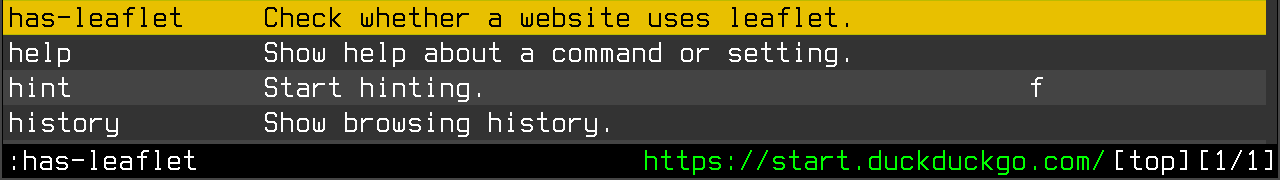
\includegraphics[width=\linewidth]{img/screenshot-completion.png}
  \caption{Command completion showing the \texttt{:has-leaflet} command.}
\end{figure}

The \py{@cmdutils.argument(...)} decorator is used to pass more information
about the \verb|tab| argument to the API. Due to the
\py{value=cmdutils.Value.cur_tab} parameter, the \verb|tab| argument is set to
the tab object of the tab currently being focused when qutebrowser calls the
command handler.

Next, the extension uses the tab API to find HTML elements on the website:

\begin{minted}[linenos,firstnumber=10]{python}
    tab.elements.find_css('.leaflet-container',
                          callback=show_message,
                          error_cb=show_error_message)
\end{minted}

The \verb|find_css()| method takes three arguments: A CSS selector, a callback
which gets called on success, and a callback which gets called in case of an
error.

The CSS class selector \verb|.leaflet-container| is used to find websites using
Leaflet, as the library uses that selector for its map display.

The callback used for errors simply uses the \verb|message| module to show an
error message to the user:

\begin{minted}[linenos,firstnumber=15]{python}
def show_error_message(error: str) -> None:
    message.error(str(error))
\end{minted}

The callback called on success instead checks whether the \verb|elements| lists
it received contains any elements. Depending on the result, it shows the
appropriate message:

\begin{minted}[linenos,firstnumber=19]{python}
def show_message(elements: typing.List[apitypes.WebElement]) -> None:
    if elements:
        message.info("Yay, this site uses Leaflet!")
    else:
        message.info("This site does not use Leaflet...")
\end{minted}

\begin{figure}[H]
  \centering
  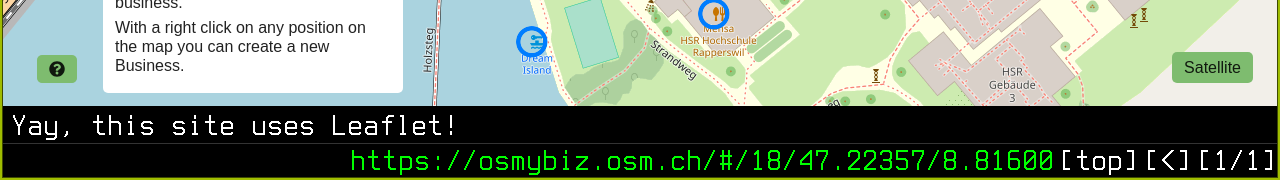
\includegraphics[width=\linewidth]{img/screenshot-leaflet.png} \\[2em]
  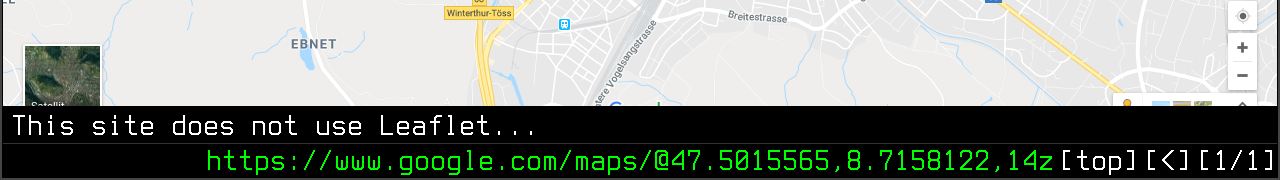
\includegraphics[width=\linewidth]{img/screenshot-leaflet-no.png}
  \caption{Results of running the \texttt{:has-leaflet} command.}
\end{figure}

Finally, the extension uses the \py{@hook.init()} decorator to define an
initialization hook. There, it displays an ``osmtest initialized'' message:

\begin{minted}[linenos,firstnumber=26]{python}
@hook.init()
def init(_context: apitypes.InitContext) -> None:
    message.info("osmtest initialized")
\end{minted}

Note that it receives an \verb|InitContext| object with additional information
(such as commandline arguments). Since the argument is unused, its name is
prefixed by an underscore, a common convention in Python code.

The full code of the demo extension can be found in listing \ref{lst:demo}.

\begin{listing}[H]
\centering
\begin{minted}[linenos]{python}
import typing

from qutebrowser.api import cmdutils, apitypes, hook, message


@cmdutils.register()
@cmdutils.argument('tab', value=cmdutils.Value.cur_tab)
def has_leaflet(tab: apitypes.Tab) -> None:
    """Check whether a website uses leaflet."""
    tab.elements.find_css('.leaflet-container',
                          callback=show_message,
                          error_cb=show_error_message)


def show_error_message(error: str) -> None:
    message.error(str(error))


def show_message(elements: typing.List[apitypes.WebElement]) -> None:
    if elements:
        message.info("Yay, this site uses Leaflet!")
    else:
        message.info("This site does not use Leaflet...")


@hook.init()
def init(_context: apitypes.InitContext) -> None:
    message.info("osmtest initialized")
\end{minted}
\caption{Demo extension}
\label{lst:demo}
\end{listing}

% Ausblick: Weiterentwicklung (nur wichtigste Punkte)
\section{Future Work}
While there was a lot of progress for extensions in qutebrowser, there is plenty
of room for future research and improvements:

\begin{itemize}
  \item The core of qutebrowser should be further modularized. Ideally, its
    architecture would be designed with the microkernel pattern \autocite[171ff]{posa1}
    for operating systems in mind, however, the resulting extension API should
    always be general enough to be useful for more than one use-case.
  \item After the extension API is stable enough, extensions should be made open
    for third-party contributions, initially by allowing users to download
    extensions they want to use in a folder such as
    \verb|~/.local/share/qutebrowser/extensions|.
  \item Many use-cases and ideas for extensions have been
    suggested\footnote{\url{https://github.com/qutebrowser/qutebrowser/issues/30}}
    by qutebrowser's users. Those should carefully be reviewed and considered
    for future API additions.
  \item In order to foster community involvement around extensions and keep
    users safe, a central place to distribute and update extensions should
    exist. Furthermore, an ``extension store'' should be added to qutebrowser,
    which allows users to easily discover, install and upgrade extensions.
\end{itemize}

The currently existing API has been designed with future additions in mind: The
\verb|downloads.py| module currently only allows triggering a temporary
download, but was split off from other modules in order to allow for future
additions for handling user-initiated downloads. Furthermore, init-hooks which
can be defined by extensions receive a special \verb|InitContext| instance
(rather than getting called with the information therein as individual
arguments) so that the \verb|InitContext| class can be extended in the future
without extensions needing to adjust their code.

% From project management part:
% % Resultate und Weiterentwicklung
% \chapter{Results and Future Work}
% 
% % Resultate (ev. nach oben in Teil I Kap. 5 eingleidern)
% \section{Results}
% 
% % Möglichkeiten der Weiterentwicklung
% \section{Possible Future Work}
% 
% % Vorgehen (welche Mögl. würde man nun wie weiterentwickeln?)
% \section{Future Approach}



% Persönliche Berichte
\section{Personal Review}

% Dank
\section{Acknowledgements}
Working on an open-source project with an idea contributed by a student, as well
as doing an SA as a single person, is rather untypical. I'm very grateful that
Prof.~Stefan~Keller was open to mentor this project as an advisor despite the
unusual conditions. His support and insights in our regular meetings were
invaluable.

Thanks to the qutebrowser community for making qutebrowser into far more than
just a personal pet project of mine. Without this community, I doubt I would
still be working on it after five years -- when I started, I never imagined that
it would get that far.

I'm thankful to all qutebrowser contributors for their patience and
understanding when I couldn't attend to their contributions in a timely manner
while working on this project. I'd especially like to thank Fritz~Reichwald for
his contributions towards switching to the Sphinx documentation generator, and
our careful coordination in order to not interfere with my own work on this
project. \fixme{update}

Thanks to AnneMarie~O'Neill for her careful English reviews and constructive
feedback on possible improvements. Her suggestions were always very welcome and
accurate.

Last but not least, thanks to Méline~Sieber for her constant encouragement
throughout the semester, and for always helping me out of the maze when I got
stuck somewhere.



\begin{appendices}
\chapter{Glossary and Abbreviations}
\begin{multicols}{2}
\label{ch:glossary}
\begin{description}[leftmargin=0pt]
  \item[API]{Application Programming Interface, i.e., in
      case of an extension API, the functions and classes (names, arguments,
      etc.) an extension can implement.}
  \item[add-on]{A synonym for \emph{extension}.}
  \item[backend]{The software library doing the ``heavy lifting'' in
      qutebrowser, such as doing network requests or drawing website content.}
  \item[CI]{Continuous integration, i.e., running automated tests or other
      checks with every change.}
  \item[DOM]{Document Object Model, the \emph{API} to access a HTML document as
      a tree structure.}
  \item[extension]{Code using an \emph{API} in order to extend the functionality
      of an existing project.}
  \item[GUI]{Graphical User Interface}
  \item[HSR]{The Hochschule für Technik (University of Applied Sciences) in
      Rapperswil, Switzerland.}
  \item[IDE]{Integrated Development Environment -- a software application
      providing tools (such as a source editor) for development.}
  \item[IFS]{The Institute for Software at \emph{HSR}.}
  \item[plugin]{In most contexts, the same as an \emph{extension}. Note that
      qutebrowser initially used \emph{plugin API} to refer to its extension
      API. However, this should be avoided, as ``plugin'' is too ambiguous in
      the context of web browsers: A plugin usually refers to software using the
      deprecated NPAPI (Netscape Plugin API) or PPAPI (Pepper Plugin API)
      technologies, such as Adobe Flash.}
  \item[Python]{The programming language used to write qutebrowser.}
  \item[PyQt]{A software library which allows to use \emph{Qt} from \emph{Python}.}
  \item[Qt]{The \emph{GUI} library used by qutebrowser}
  \item[QtWebEngine]{The \emph{backend} used by default in qutebrowser, based on
      the Chromium project (like the Chrome web browser).}
  \item[QtWebKit]{One of two possible \emph{backends} qutebrowser can use.
      QtWebKit is the older backend, which isn't used by default anymore, but is
      still supported.}
  \item[SA]{Studienarbeit (Student research project)}
  \item[W3C]{World Wide Web Consortium, the standards body for web-related
      technologies such as HTML.}
\end{description}
\end{multicols}

\chapter{API documentation}
\label{ch:sphinx}
\fixme{some text}
\includepdf[pages=5-18,trim=0 2cm 0 1.8cm,clip,pagecommand=,offset=0 1cm]{./img/sphinx.pdf}

\chapter{Test log}
\label{ch:testlog}
\begin{minted}{text}
========================== test session starts ==========================
platform linux -- Python 3.7.1, pytest-4.0.1, py-1.7.0, pluggy-0.8.0
cachedir: .tox/py37/.pytest_cache
PyQt5 5.11.3 -- Qt runtime 5.12.0 -- Qt compiled 5.12.0
benchmark: 3.1.1 (defaults: [...])
hypothesis profile 'default' -> [...]
rootdir: /home/florian/proj/qutebrowser/git, inifile: pytest.ini
plugins: xvfb-1.1.0, travis-fold-1.3.0, rerunfailures-5.0, repeat-0.7.0,
  qt-3.2.1, mock-1.10.0, instafail-0.4.0, faulthandler-1.5.0, cov-2.6.0,
  benchmark-3.1.1, bdd-3.0.0, hypothesis-3.82.5
collected 195 items

tests/unit/api/test_cmdutils.py ..........................................
                                ...................
tests/unit/components/test_adblock.py ..............................
tests/unit/components/test_misccommands.py .....
tests/unit/extensions/test_loader.py ............
tests/unit/browser/webengine/test_webenginetab.py .....
tests/end2end/features/test_caret_bdd.py ...........
tests/end2end/features/test_scroll_bdd.py ..................s.............
                                          ...................
tests/end2end/features/test_zoom_bdd.py ...............x....


--------------- benchmark: 1 tests ---------------
Name (time in us)             Min      Max  Median
--------------------------------------------------
test_adblock_benchmark     3.3040  40.3980  3.4670
--------------------------------------------------

Legend:
  Outliers: 1 Standard Deviation from Mean; 1.5 IQR (InterQuartile Range)
            from 1st Quartile and 3rd Quartile.
  OPS: Operations Per Second, computed as 1 / Mean
=========== 193 passed, 1 skipped, 1 xfailed in 44.72 seconds ===========
\end{minted}

Tests marked with \emph{s}/\emph{skipped} were skipped because of
platform/environment differences. Tests marked with \emph{x}/\emph{xfailed} were
expected to fail due to known bugs.

Note only the subset of tests relevant to this project was ran.

\renewcommand{\bibname}{\chapter{Literature and Sources}}
\printbibliography
\end{appendices}

\end{document}
